\documentclass[11pt]{article}
\usepackage[utf8]{inputenc}
\usepackage[margin=1in]{geometry}
\usepackage{natbib,graphicx,mdframed,hyperref,threeparttable,amssymb}



\title{An agent-based model for city networks based on interactions between firms}

\date{}

\begin{document}

\author{J. Raimbault$^{1,2,3,\ast}$, N. Zdanowska$^{1,3}$ and E. Arcaute$^1$\\\medskip\small
$^{1}$ Centre for Advanced Spatial Analysis, UCL; $^{2}$ UPS CNRS 3611 ISC-PIF; $^{3}$ UMR CNRS 8504 G{\'e}ographie-cit{\'e}s\\
$^{\ast}$ \texttt{juste.raimbault@polytechnique.edu}
}

\maketitle
% NetSci format: A4, 11pt, 1in margin, max 12p + up to 3p references

\begin{abstract}
    This paper introduces a generative model for urban networks defined by interactions between firms to test several geographical properties emerging in such a network as metropolisation or internationalisation. The growth of the network is simulated by adding randomly new links defined by ownership between firms, with probabilities of occurring depending on the economic size of urban areas at origin and destination, industrial sector proximity between firms, the strength of links from the past as well as the geographical and socio-cultural distance. The simulation on a synthetic system of cities unveil phase transitions when changing interaction distance, and non-trivial patterns in the model behavior. Calibration of the model on real data on company ownership linkages for Europe in 2018 is also undertaken. Future work will consist in observing thanks to this model the impact of economic crisis on such networks.
    
    
\end{abstract}

\section{Introduction}

The intensification of globalisation of the economy since the late 20th century resulted in the rise of the network society \cite{castells2000networksociety} and the emergence of a world-city system \cite{taylor2001specification}, characterized by highly interconnected urban centres at the global level \cite{sassen1991}. These interactions can be of different nature and determined by economic, socio-cultural, or geopolitical proximity implying spatial and non spatial patterns \cite{martinus2018global}. Interactions of economic nature between transnational firms, are together with trade among the most representative of the current economic trends \cite{taylor2001specification}. Understanding the drivers of growth and geographical properties of such a urban network, can be used to foster innovation in specific cities and to shape public policies for local industrial clusters \cite{turkina2016structure}. Straightening these city-interactions can be crucial for revitalising certain geographical areas \cite{Clarke2018}, by developing strategic industries for global insertion of regions \cite{dawley2019creating}, cities \cite{gluckler2016relational} and countries \cite{martinus2019brokerage}. The functioning of such a city-network and the position of cities within these networks \cite{gluckler2016relational} can also permit to infer the consequences of future exogenous shocks such as an economic crisis, a single market collapse or a post-Brexit scenario for the European Union.

The use of network models to understand processes underlying the emergence and dynamics of such urban networks has already been widely tackled in the literature. \cite{dai2016simulating} propose a generative urban network model at the regional scale, combining geographical factors with network topological properties. Air transportation networks can also be understood as urban networks, and \cite{zanin2013modelling} reviews several models for such networks. Trade network have been extensively studied from complex networks perspective, but are generally driven at the country-level \cite{garlaschelli2005structure} because of lack of city-level data. Input-output models, mostly used in regional science to represent flows between geographical areas, are considered in some cases as a type of urban generative model \cite{jin1993generation}. In this stream of research, spatial interaction models \cite{dennett2013multilevel} can form the basis of urban network models for abstract flows \cite{dai2016generative} or physical infrastructure \cite{raimbault2020indirect}.




%\citep{martinus2018global} combination of different types of proximity in inter-urban firm networks: economic, sociocultural, geopolitical - implies spatial and non-spatial 
%\citep{pan2017mapping} different types of linkages: e.g. services here, but not only. All sectors should be taken into account first.
%\cite{martinus2019brokerage} role of small countries
%\cite{dawley2019creating} regional policies for insertion in global network
%\cite{gluckler2016relational} positioning within networks

In this paper we choose to focus on urban networks of firms to question how can we understand and capture geographical and economic processes as agglomeration economies \cite{Glaeser2001} characteristic to spatial economy \cite{Fujitaetal2001} within a generative model. The originality of the present paper is to approach these issues within the system of cities framework \cite{berry1964cities}, where the position and dynamics of cities in the socio-economic world-wide space can be considered by their interactions with other cities \cite{pumain2018evolutionary}. We examine the interactions of European cities within firm linkages defined by corporate ownership links. Since transnational firms structure is one of the determinant of the global economic space, it provides one accurate proxy to unveil geographical structures \cite{2019arXiv191014652Z}. 

More precisely, our contribution relies on the following points: (i) we propose an empirical analysis of the firm ownership urban network for the European Union, based on the Bureau Van Dijk's \emph {AMADEUS} database; (ii) we introduce a generative network model to simulate the growth of such linkages at urban areas scale, which combines multiple factors influencing link formation, as economic intensity of origin and destination of urban areas, industrial sector proximity, the strength of previous links, and geographical and socio-cultural distance; (iii) the model allows us to compare the effect of different factors on the final network structure, which is extensively studied through model sensitivity analysis and exploration; and (iv) we calibrate the model on the empirical network.


The rest of this paper is organized as follows: we first proceed to an empirical analysis of the network studied. We then describe the generative model for urban networks, and its sensitivity analysis and exploration on synthetic data. We then parametrize and calibrate the model on real European firm ownership data. We finally discuss implications of our results and possible extensions.


\section{Empirical network analysis}

% stats to describe the structure of the database, nb of total links, nodes, missing values? + nb of firms per country,  total turnover generated per country etc..

Companies from the AMADEUS database are georeferenced using the Geonames database (using postcode or address depending on the information available). We then join this data with the GHS-FUA dataset for Functional Urban Areas \cite{Florczyk2019ghs}, which are the most relevant objects for applying our model. Starting from a firm-level dataset of 1,562,862 nodes and  1,866,936 links, we obtain a directed network of 573 urban areas and 9323 ownership links. Weight of links are obtained by computing the owned share of turnover at destination, i.e. $w_{ij} = \sum_{k \in i,l \in j} p_{kl} \cdot T_l$ where $p_{kl}$ of the ownership share of company $l$ by company $k$ and $T_l$ the turnover of company $l$. Node attributes include an economic size of urban areas, that we compute as the sum of turnovers of companies within the area. This quantity is highly correlated with area-level GDP included in the GHS database (Spearman correlation $\rho = 0.71$) and also with population ($\rho = 0.60$), so we expect to capture size effects while keeping the consistence of a single main data source. An other attribute of nodes is the industrial sector composition, expressed as a proportion of turnover in the area associated to a given industrial sector. Detailed sectors of firms are available up to the four digits of the NACE classification in the raw data. We consider the first level classification (21 categories) and compute sector proportions accordingly. This allows us to define an industrial proximity matrix between urban areas, taking a cosine similarity between vectors as $s_{ij} = \sum_{k=1}^{K} S_{ik}\cdot S_{jk}$ where $S_{ik}$ are sector proportions.


The urban network has heavy tail weighted degree and edge weight distributions, as shown in Fig.~\ref{fig:nwdist}. We fit power law and log-normal distributions, including minimal value cutoff following \cite{clauset2009power}, using the \texttt{powerlaw} R package \cite{powerlawpackage}. For both, log-normal distributions appear to be a better fit ($\mu=18.8$, $\sigma=2.3$ for weighted degree; $\mu=13.8$, $\sigma=2.8$ for edge weight), and include a much broader range of the empirical distributions with lower estimated cut-offs. These heavy tail properties suggest the relevance of a generative model including self-reinforcing processes which are known to produce such distributions.

%%%%%%%%%%%%%
\begin{figure}
    \centering
    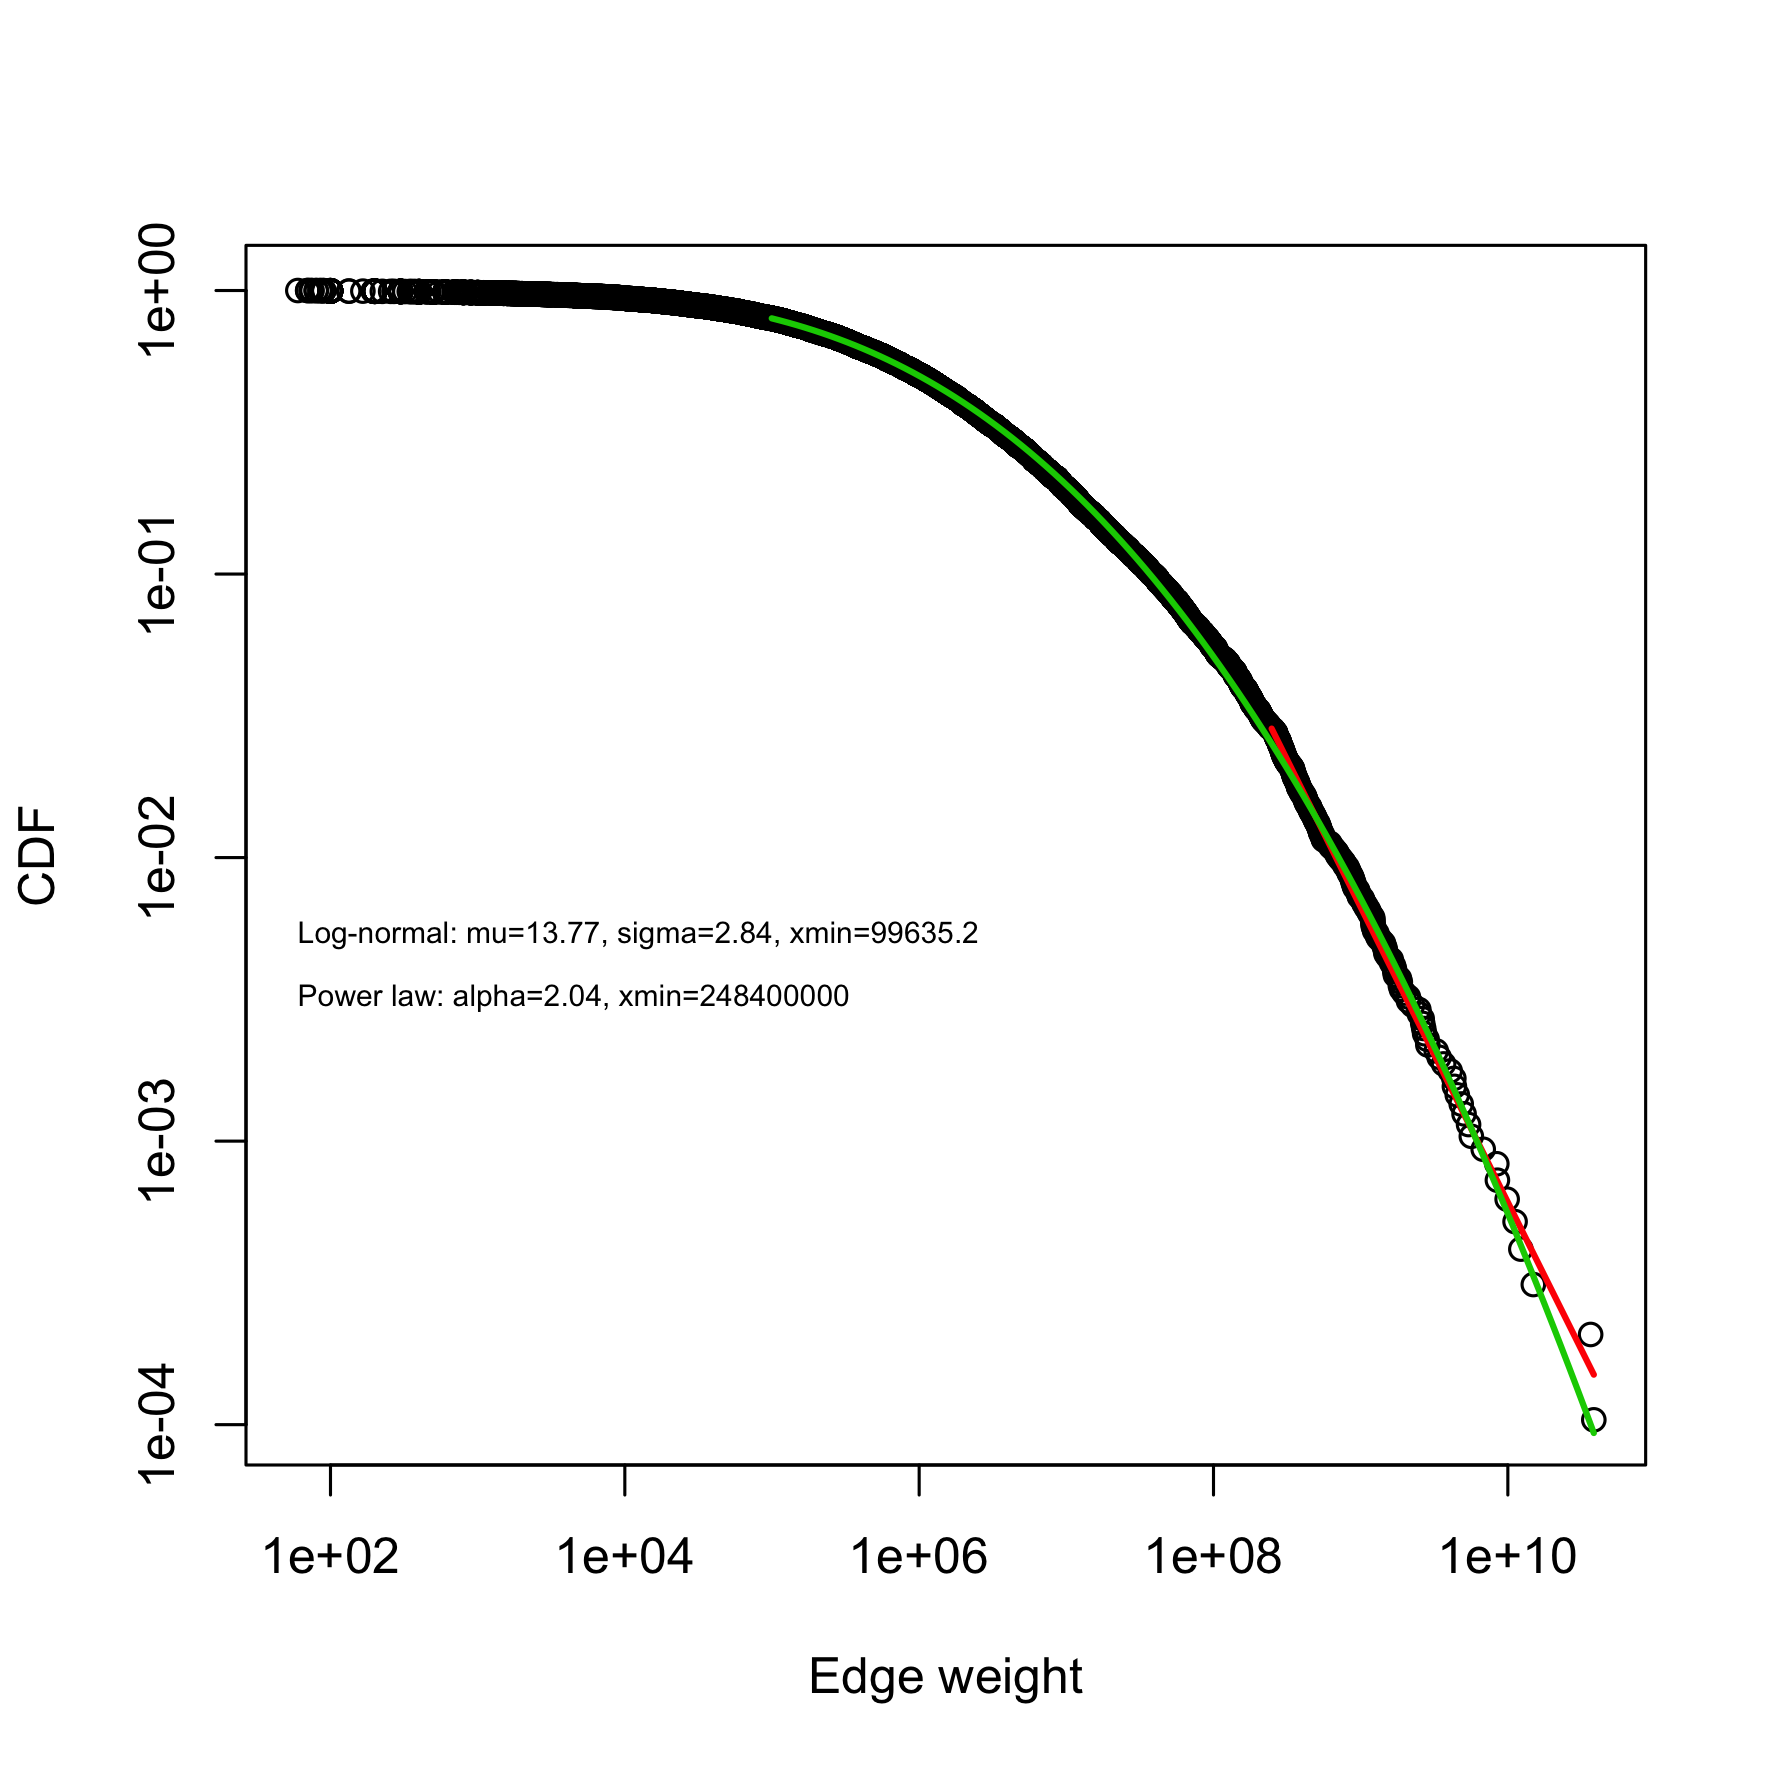
\includegraphics[width=0.49\textwidth]{figures/edgeweight.png}
    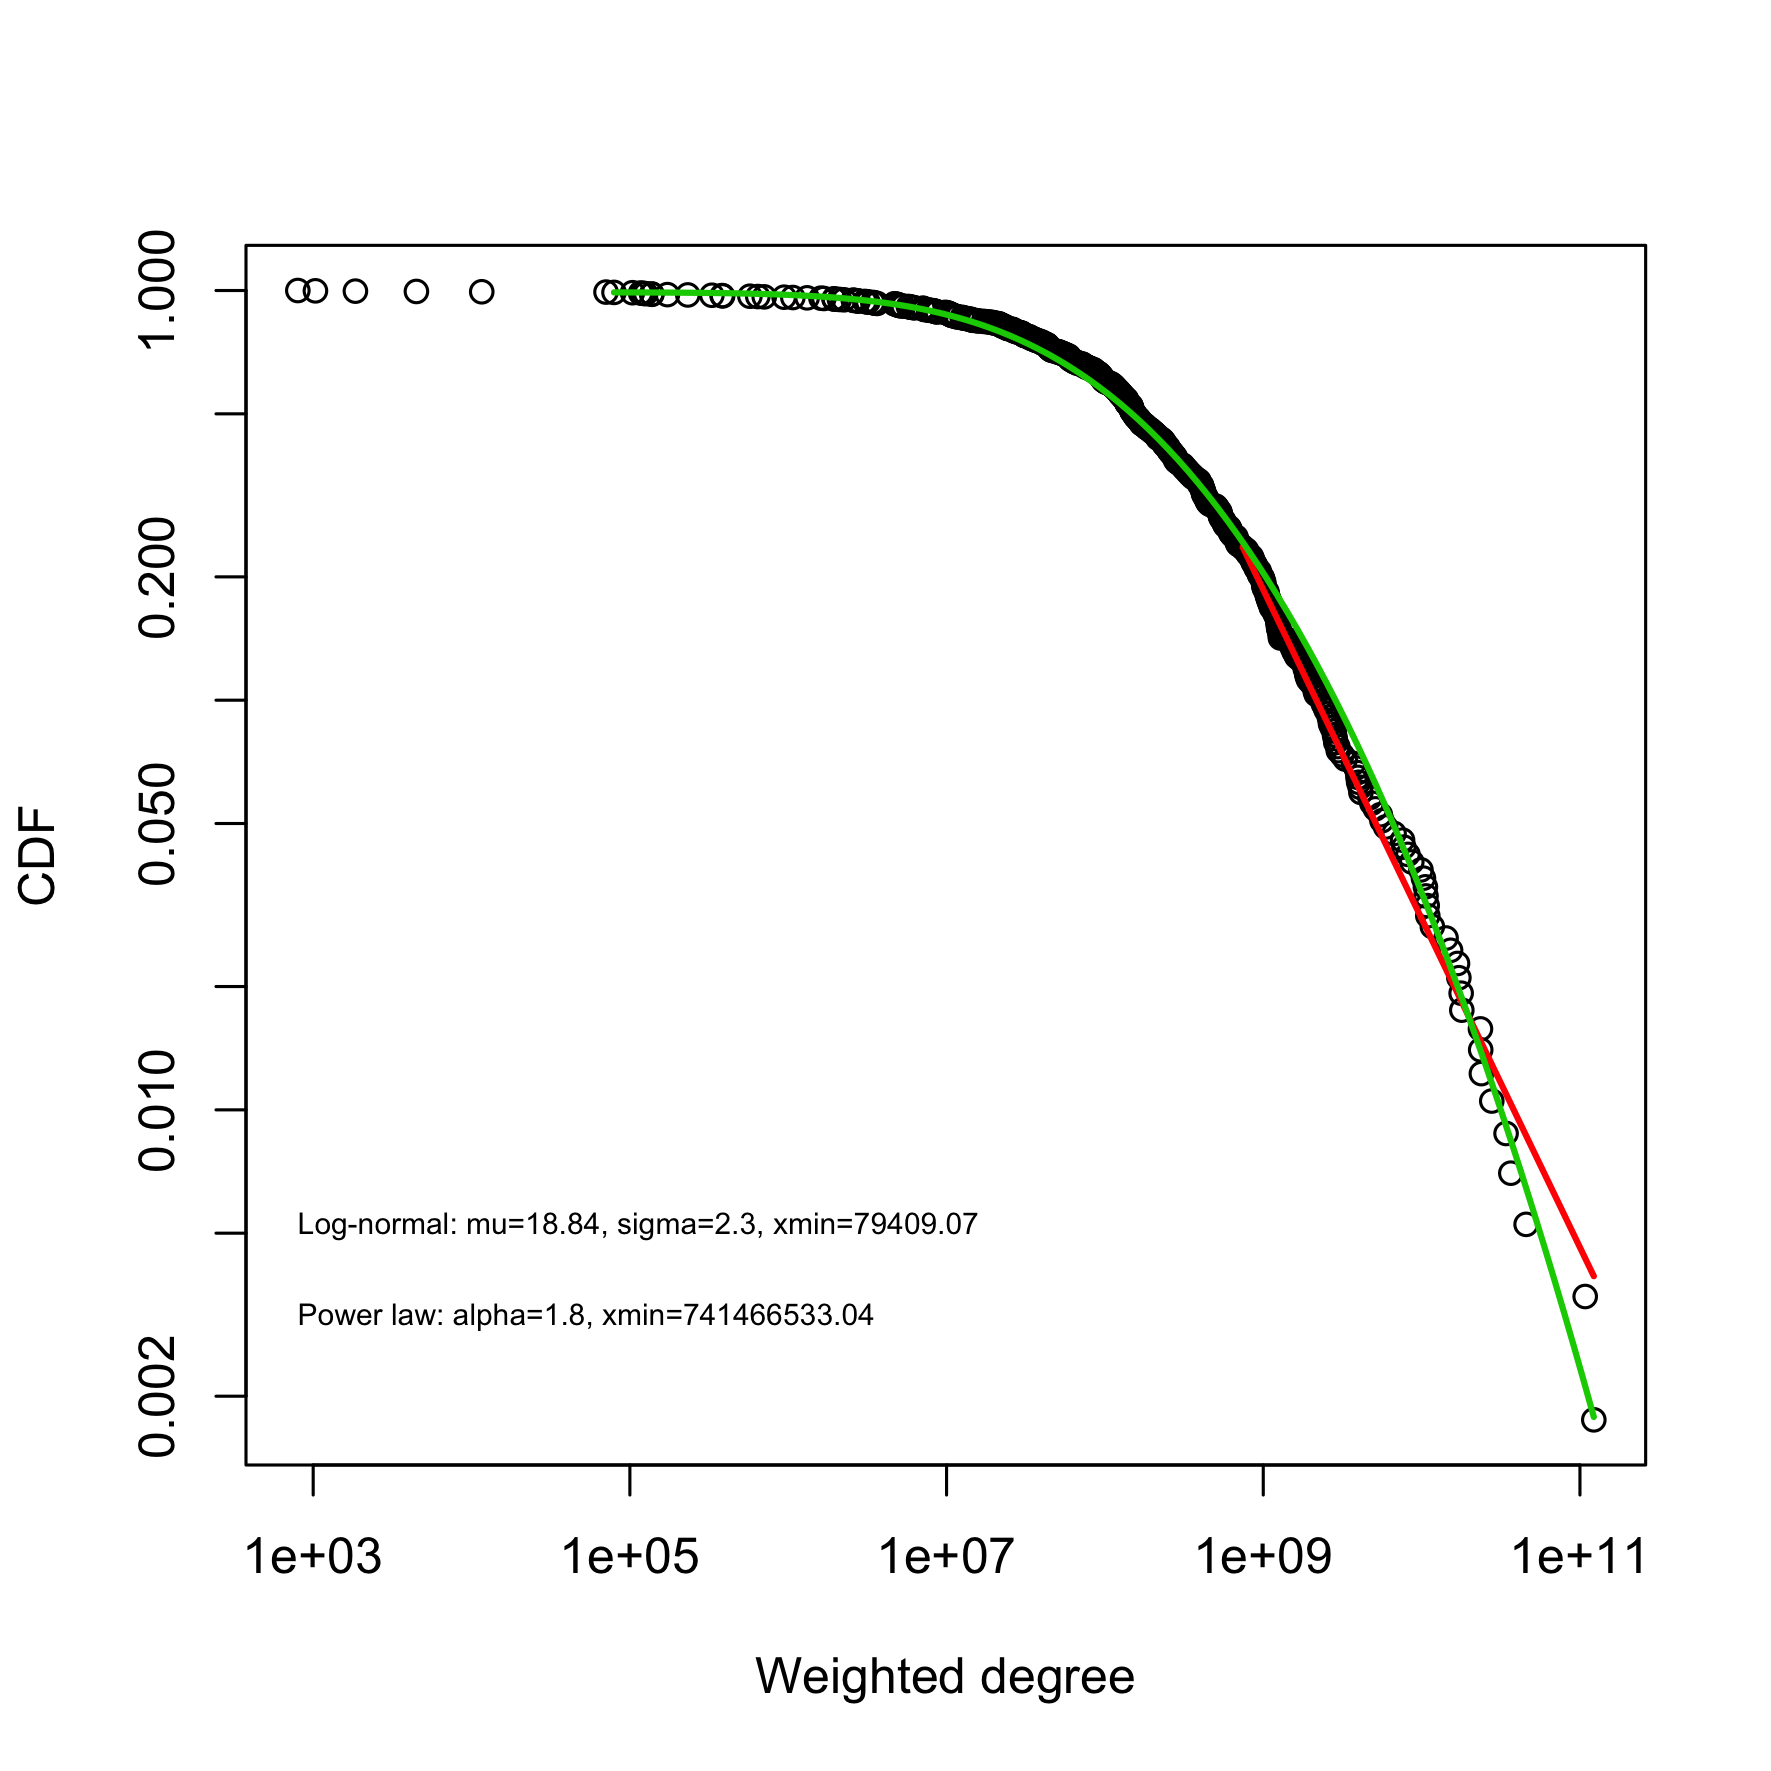
\includegraphics[width=0.49\textwidth]{figures/degreeDistr.png}
    \caption{Distributions of network properties. \textit{(Left)} Cumulated distribution for edge weight, with power law fit (red) and log-normal fit (green); \textit{(Right)} Cumulated distribution for weighted degree.}
    \label{fig:nwdist}
\end{figure}
%%%%%%%%%%%%%


Regarding the community structure of the network, different modularity maximisation algorithms (run on the undirected corresponding network) give a same undirected modularity of 0.38, and a directed modularity \cite{nicosia2009extending} of 0.34 for the greedy algorithm of \cite{clauset2004finding} and 0.36 for the Louvain algorithm \cite{blondel2008fast}, corresponding to 36 communities (resp. 15). In comparison, with 29 countries, the classification of urban areas by country has a modularity of 0.32. This means that the structure of flows present certain regional patterns. Indeed, a null model assigning random labels with 30 communities, bootstrap 1000 times, yields an average modularity of $0.049 \pm 0.002$, confirming the statistical significance of these communities.


To have a first insight into factors playing a role in the formation of links, we proceed to a statistical analysis similar to unconstrained spatial interaction models \cite{wilson1975some}. We test five different statistical models, including progressively the processes candidate to be included in the network generative model. The most general statistical model is
\[
\log(w_{ij}) = \log(d_{ij}) + \log(T_i) + \log(T_j) + \log(s_{ij}) + \alpha_{c_i,c_j} + \varepsilon_{ij}
\]
where $\alpha_{c_i,c_j}$ is a fixed effect term for the couple of countries $c_i,c_j$. We use a multiplicative form by taking logarithms as it is usually done for spatial interaction models. Furthermore, origin and/or destination constrained models are not relevant in our case as links include not only turnover but also a share of ownership. Estimation results are given in Table~\ref{tab:reg}. We also fit a Poisson generalized linear model with a logarithmic link on the rounded weights \cite{flowerdew1988fitting}. We find that distance alone (model 1) has a significant negative effect but with an explained variance close to zero. The second model adds fixed effects by pair of countries, for which around a third are significant, and with a better $R^2$ of 0.17. Adding origin and destination economic size (turnovers $T_i$ and $T$, model 3) slightly improves the explanative power, but the best model among the linear ones is the model 4 with all factors and fixed effects, both in terms of explained variance ($R^2 = 0.31$) and Akaike information criterion. The latter indicates the absence of overfitting. The Poisson model with all variables is much better regarding pseudo-$R^2$ and provides much more significant estimates (all fixed effects significant and much smaller standard deviations). Across all models, we find consistent qualitative stylized facts: (i) distance has a negative influence; (ii) economic sizes have a positive influence, with the size of the origin being more important (what is consistent with ownership links, strongly driven by decision at the headquarters); (iii) industrial proximity has a positive influence, i.e. similarity is more important than complementarity for this dimension; (iv) an important part of country fixed-effects are significant; and (v) the order of magnitude of the influence of each factor is roughly the same, in the sense that no process totally dominates the others. This suggests the relevance of including all these different dimensions in the generative network model.


%%%%%%%%%%%%%
\begin{table}[h]
\caption{Ordinary Least Square estimations of statistical models explaining $\log(w_{ij})$ (standard errors in parenthesis). ***, ** and * respectively indicate 0.01, 0.05 and 0.1 levels of significance. For the fixed effect by origin-destination pairs of countries, we give the proportion of significant coefficients (where $p<0.1$). Models (1) to (4) are ordinary least square models, while model (5) is a Poisson generalized linear model with logarithmic link. We compare model performance using $R^2$, Mean Square Error, and Akaike Information Criterion. For the Poisson model, AIC is not given as it is not comparable, and the pseudo-$R^2$ is given either.\label{tab:reg}}
\medskip
\begin{tabular}{|l|c|c|c|c|c|}
\hline
Model  & (1) & (2) & (3) & (4) & (5) \\ 
\hline
$\log(d_{ij})$ &      -0.06** (0.03) &   -0.11** (0.05)  & -0.41*** (0.02)  & -0.35*** (0.04)  &  -0.26*** ($5\cdot 10^{-6}$) \\
$\log(T_i)$ &   &   & 0.56*** (0.01) &  0.56*** (0.01) & 0.79*** ($2\cdot 10^{-6}$) \\
$\log(T_j)$ &     &   & 0.39*** (0.01) &  0.39*** (0.01) & 0.66***  ($1.5\cdot 10^{-6}$) \\
$\log(s_{ij})$ &     &   &  &  0.19*** (0.07) & 0.53*** ($9\cdot 10^{-6}$)  \\
Countries &    &  28.3\% &   &  26.5\% & 100\% \\
\hline
$R^2$ &       0.00059   &  0.17 & 0.21 &  0.31  &  0.56 \\
MSE & 7.75 & 6.84 & 6.10 & 5.33 & 8.72 \\
AIC &        44304   &  43578  &  42131  & 41917 &   \\
\hline
\end{tabular}
\end{table}
%%%%%%%%%%%%%



\section{Model}

\subsection{Rationale}

The model is expected to capture a single macroscopic urban scale, i.e. the level of the urban system where basic entities are cities. Links are induced by underlying firms but these are not explicit. Cities are defined by their economic size, but also by an industrial sector profile. As \cite{martinus2018global} point out, a combination of several distances may play a role in establishing linkages. Geographical distance, industrial proximity and complementarity will typically be equally significant \cite{cottineau2020nested}. Therefore, we combine several processes driving network growth: (i) geographical proximity (in our case the crow-fly distance, but it can be generalized to any type of accessibility); (ii) geopolitical proximity, which captures the higher propensity to establish links within existing submarkets despite the European common market (confirmed relevant by the fixed effect regression described above); (iii) city economic size, which has furthermore scaling laws properties; (iv) industrial proximity in terms of firm sector composition; (v) previous linkages (influence of history). This last point is crucial to capture accumulated effects and include path-dependency, which fits well the use of a simulation model instead of a more simple statistical model.



\subsection{Model description}

Let $1 \leq i \leq N$ cities defined at time $t$ by their economic structure such that $E_i(t)$ is the total economic volume (GDP) for city $i$ and $S_{ik}(t)$ is a matrix giving economic volume proportions within each economic sector $k$, assuming $K$ economic sectors. Formally, the model creates links between cities which are characterized by their economic size $E_i$ (GDP) and economic structure $S_{ik}$ in terms of activity sectors (probability distribution of firms within $K$ sectors). Starting with an existing network with no links, the model iteratively adds links, following a probability given by a generalized Cobb-Douglas function \cite{vilcu2011geometric} as 

\begin{equation}
p_{ij} \propto \left(\frac{E_{i}}{E}\right)^{\gamma_F} \cdot \left(\frac{E_{j}}{E}\right)^{\gamma_T} \cdot \left(\frac{w_{ij}}{W}\right)^{\gamma_W} \cdot s\left(S_{ik},S_{jk}\right)^{\gamma_S} \cdot \exp \left(- \gamma_G \cdot d_{ij}\right) \cdot \exp \left(- \gamma_D \cdot g_{ij}\right)
\end{equation}

where $E  =  \sum_k E_k$, $W  = \sum_{i,j} w_{ij}$ weights of previous links, $s(S_{ik},S_{jk})$ is a similarity function between activity sectors $S_{ik}$ and $S_{jk}$ taken as a cosine similarity, $d_{ij}$ euclidian distance, and $g_{ij}$ a socio-cultural distance. In the case of an already existing link between two areas, the weight of the latter is incremented by a unit volume $w_0$. The model is stopped either when a final time is reached or when the cumulated volume of links reaches a target quantity. This formulation can be considered both as an economic utility model and a generalisation of spatial interaction models.



Note that: (i) we consider an asymmetric influence of sizes, assuming that link directions are important (similarly the similarity function $s$ may be taken as asymmetric); (ii) the influence of previous links is similar to a preferential attachment process; (iii) we do not renormalize the exponents to 1 (which is different than renormalising the probability), to ensure to include convex functions. The ``geopolitical/sociocultural'' distance remains abstract and should be parametrised (see setup below) and estimated in the data-driven setting. We assume no evolution of economic size in this simple version of the model, which means that adjusted parameter are valid on a restricted time period.


\subsection{Model setup}

Besides model dynamics, its initialisation (or parametrisation on real data) regarding the spatial distribution, sizes, countries and industrial sector compositions, is also important to understand model behavior. In addition  \cite{raimbault2019space} showed that the initial spatial configuration can have significant impacts on model outcomes. We therefore consider two versions: one with a synthetic system of cities which can be stochastically repeated, and one other based on real data.


\paragraph{Synthetic setup}

The synthetic system of cities is generated to be at the scale of a continent with properties similar to Europe: (i) $N=700$ cities with an empirical power-law from the Global Human Settlements database for economic sizes ($\alpha = 1.1$), distributed randomly into a uniform and isotropic square space of width $d_{max}=3000km$; (ii) clustered into $C = 20$ countries using a k-means algorithm (this remains consistent with non-correlated city sizes at the scale of the countries as our cities are randomly distributed in space \citep{simini2019testing}); (iii) with synthetic distribution of sectors following log-normal distributions adjusted in a way that large cities have more high-value activities and are more diverse. More precisely for this last point, assuming sectors are distributed continuously along a one-dimensional axis, cities are assumed to have a sector distribution with a log-normal density function. The largest city is constrained to have a standard deviation and a mode of $1/2$ and the smallest $1/K$, with a linear interpolation between the two for other cities. Parameters of the log-normal law are obtained by solving the corresponding two equations system for each city, and each distribution is discretised and renormalised to be a vector of probabilities. In synthetic experiments, the network is generated from an empty initial network until reaching $t_f=1500$, with a unit link volume of $w_0 = 1$.

     
\paragraph{Real setup}

The real setup is done using the empirical network analyzed above. Urban areas are distributed according to their positions in the actual geographical space, and economic size and sector composition attributes are used. The socio-economic distance is constructed using information from the statistical modeling, by considering fixed-effect coefficients estimated for each pair of countries. Initial network is empty, and the real links are taken as targets for the generated network. We constrain the total volume of flows by setting $w_0 = \sum_{ij} w_{ij} / t_{f}$ when the number of time steps $t_f$ is given as a parameter.


\subsection{Model parameters and indicators}


The model parameters are the Cobb-Douglas weights $\gamma_F,\gamma_T,\gamma_W,\gamma_s$ and distance decay parameters $\gamma_G,\gamma_D$. The model also includes path-dependency by integrating the influence of previous links. Therefore it can not be reduced to a simple statistical model. Finally, the role of space introduces even further complexity, yielding a generative model, which has to be simulated.

We consider several macroscopic indicators to quantify the generated network. Firstly, geographical structures are captured by (i) internationalisation (modularity of countries in the network); (ii) metropolisation (correlation between weighted degree and city size). Two other thematic indicators, which are regionalisation (correlation between length and flow of links, stratified by size of extremities), and specialisation (correlation between sector proximity and flow of links, stratified by size of extremities), are not included in this study for the sake of simplicity as each has a high dimension. We also consider several network indicators as Louvain modularity, sizes of maximal modularity communities, degree and link weight distributions (described by their average, hierarchy, and entropy), and correlations between degree and city size, and between link weight and distance.



\section{Model exploration and calibration}

The model is implemented in NetLogo, which provides a good compromise between performance and interactive prototyping and exploration \cite{railsback2017improving}. Numerical experiments are done by integrating the model into the OpenMOLE software for model exploration \cite{reuillon2013openmole}, which provides sensitivity analysis and calibration methods and a transparent access to high-performance computing infrastructures. Model source code, aggregated network data (raw initial firm network can not be made available for data ownership reasons), and results are available on the open Git repository of the project at \url{https://github.com/JusteRaimbault/ABMCitiesFirms}. Large simulation result files are available on the dataverse repository at \url{https://doi.org/10.7910/DVN/UPX23S}. We show in Fig.~\ref{fig:example} examples of generated networks, with very contrasted patterns obtained with different spatial interaction ranges. Low values of the gravity decay parameter yield local networks around main cities, while long interaction ranges yield more integrated networks. We also show networks simulated in the real setting.

%%%%%%%%%%%%%
\begin{figure}
    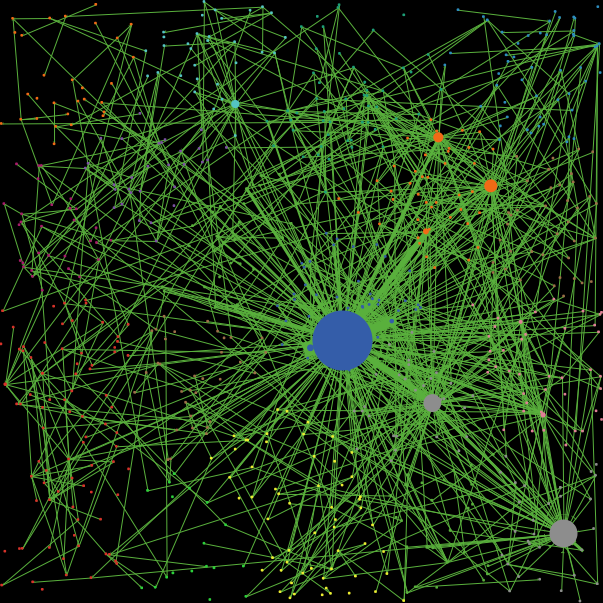
\includegraphics[width=0.48\textwidth]{figures/ex_alleq-highgravity_seed-12102_t1500.png}
    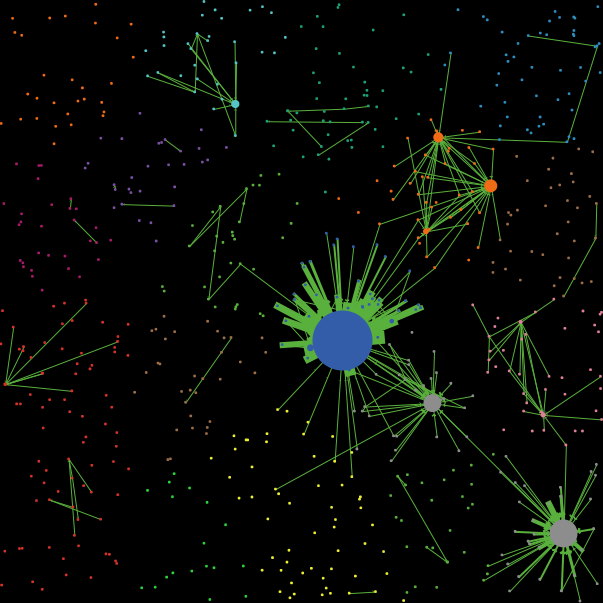
\includegraphics[width=0.48\textwidth]{figures/ex_alleq-lowgravity_seed-12102_t1500.png}\\
    \begin{minipage}{0.48\textwidth}
    \begin{mdframed}
    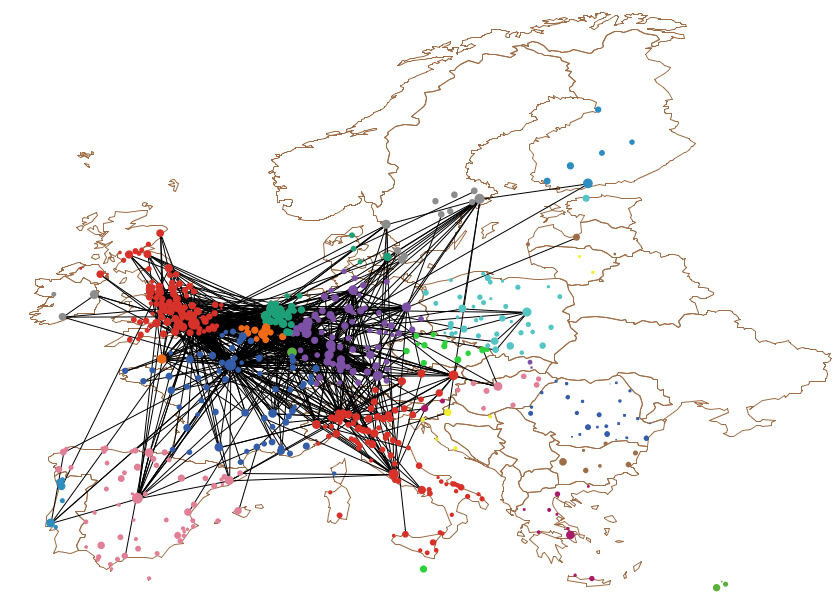
\includegraphics[width=\textwidth]{figures/ex_real_highgravity_t1500.png}
    \end{mdframed}
    \end{minipage}
    \begin{minipage}{0.48\textwidth}
    \begin{mdframed}
    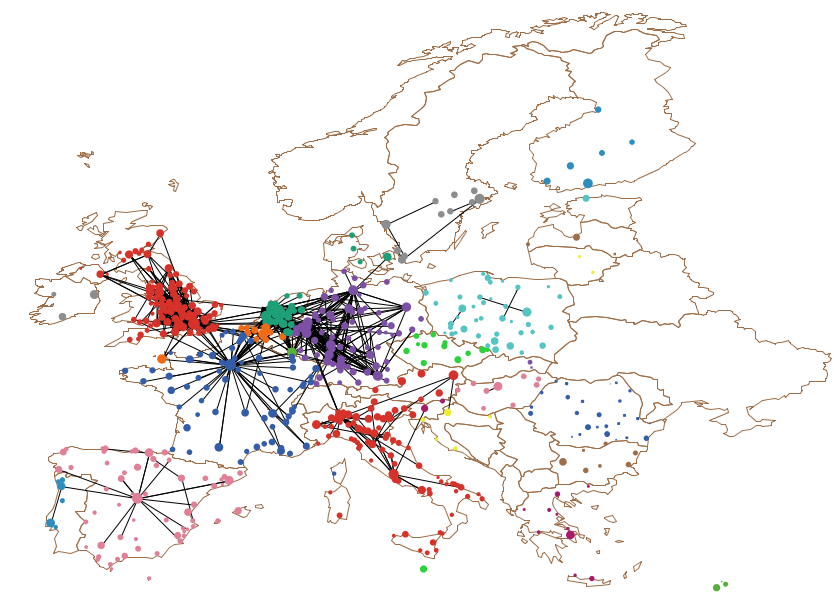
\includegraphics[width=\textwidth]{figures/ex_real_lowgravity_t1500.png}
    \end{mdframed}
    \end{minipage}
    \caption{Example of simulated networks at $t=1500$, for a synthetic system of cities (Top row) and the European urban network (Bottom row). , with a high (resp. low) gravity decay parameter for the left column (resp. right).\label{fig:example}}
\end{figure}
%%%%%%%%%%%%%


\subsection{Synthetic city systems}

We first study extensively the behavior of the model on synthetic systems of cities, to isolate its intrinsic behavior independently of a contingent geographical situation.

\paragraph{Sensitivity analysis}

A global sensitivity analysis first unveils an aggregated influence of parameters on model indicators. We apply Saltelli's Global Sensitivity method introduced by \cite{saltelli2008global}. This produces values for each parameter and each output of a first order sensitivity index, defined as $Var\left[\mathbb{E}_{\mathbf{X}_{\sim i}}\left(Y_j | X_i\right)\right] / Var\left[Y\right]$, for parameter $X_i$ and output $Y_j$, $\mathbf{X}_{\sim i}$ being all other parameters. This captures the total influence of $X_i$ all other things being equal. The total order index is given by $\mathbb{E}_{\mathbf{X}_{\sim i}} \left[Var(Y_j | \mathbf{X}_{\sim i})\right] / Var\left[Y_j\right]$ and captures non-homogeneity in behavior and interaction between parameters. Indices were estimated with a Sobol sequence sampling of 20,000 model runs \cite{saltelli2010variance}. We give in Table~\ref{tab:saltelli} estimated results. We find that indicators related to modularity (internationalisation and optimal modularity) are mostly influenced by geographical parameters. On the contrary, indicators of network structure are driven by origin and destination sizes. Sectors and link history have a second order by not negligible role. Altogether, the analysis witnesses of strong interaction effects between parameters, since for several indicators the total order index is one order of magnitude larger than the first order index. This means that the generative model captures some complex behavior of the system. The very different important parameters depending on outputs studied confirms the relevance of a more exhaustive grid exploration.


%%%%%%%%%%%%%
\begin{table}
\caption{Saltelli sensitivity indices, for indicators in rows and parameters in columns. We give for each pair the first order index (F) and the total order index (T).\label{tab:saltelli}}
\hspace{-1cm}\begin{tabular}{|l|c|c|c|c|c|c|c|c|c|c|c|c|}
\hline
 & \multicolumn{2}{|c|}{$\gamma_G$} & \multicolumn{2}{|c|}{$\gamma_D$} & \multicolumn{2}{|c|}{$\gamma_S$} & \multicolumn{2}{|c|}{$\gamma_W$} & \multicolumn{2}{|c|}{$\gamma_F$} & \multicolumn{2}{|c|}{$\gamma_T$} \\
 & F & T & F & T & F & T & F & T & F & T & F & T \\
 \hline
Internationalisation & 0.2 & 0.3 & 0.7 & 0.7 & 0.001 & 0.009 & $4\cdot 10^{-4}$ & 0.007 & 0.03 & 0.04 & 0.02 & 0.04 \\
Metropolisation & 0.02 & 0.1 & 0.02 & 0.2 & 0.002 & 0.1 & 0.001 & 0.09 & 0.2 & 0.6 & 0.3 & 0.6 \\
Modularity & 0.3 & 0.4 & 0.6 & 0.6 & 0.004 & 0.02 & $3\cdot 10^{-4}$ & 0.01 & 0.005 & 0.03 & 0.002 & 0.03 \\
Avg. com. size & 0.008 & 0.09 & 0.01 & 0.1 & 0.002 & 0.07 & 0.003 & 0.04 & 0.3 & 0.6 & 0.4 & 0.6 \\
Degree entropy & 0.006 & 0.02 & 0.003 & 0.02 & 0.006 & 0.03 & 0.008 & 0.02 & 0.5 & 0.5 & 0.5 & 0.5 \\
Weight entropy & 0.04 & 0.1 & 0.03 & 0.1 & 0.008 & 0.08 & 0.01 & 0.07 & 0.4 & 0.5 & 0.4 & 0.5 \\\hline
\end{tabular}
\end{table}
%%%%%%%%%%%%%



\paragraph{One factor sampling}

A first numerical experiment of one-factor sampling on all Cobb-Douglas parameters and 100 stochastic repetitions confirms a good statistical convergence (average Sharpe ratios for indicators all larger than 5). We use thus 20 repetitions in following larger experiments (in the case of a normal distribution, a 95\% confidence interval on the average is of size $2\sigma \cdot 1.96 / \sqrt{n}$, what gives $n=16$ repetitions for a CI of width of the standard deviation). Behavior of some indicators are shown in Fig.~\ref{fig:onefactor}. For example, internationalization and the correlation between economic size and weighted degree both show a phase transition as a function of $\gamma_G$, from a local to a global regime. The sector proximity parameter $\gamma_S$ influences the internationalization linearly, but induces a maximum for the correlation between size and degree, which can be interpreted as a setting where size and the total volume in a city are the most correlated.

%%%%%%%%%%%%%
\begin{figure}
	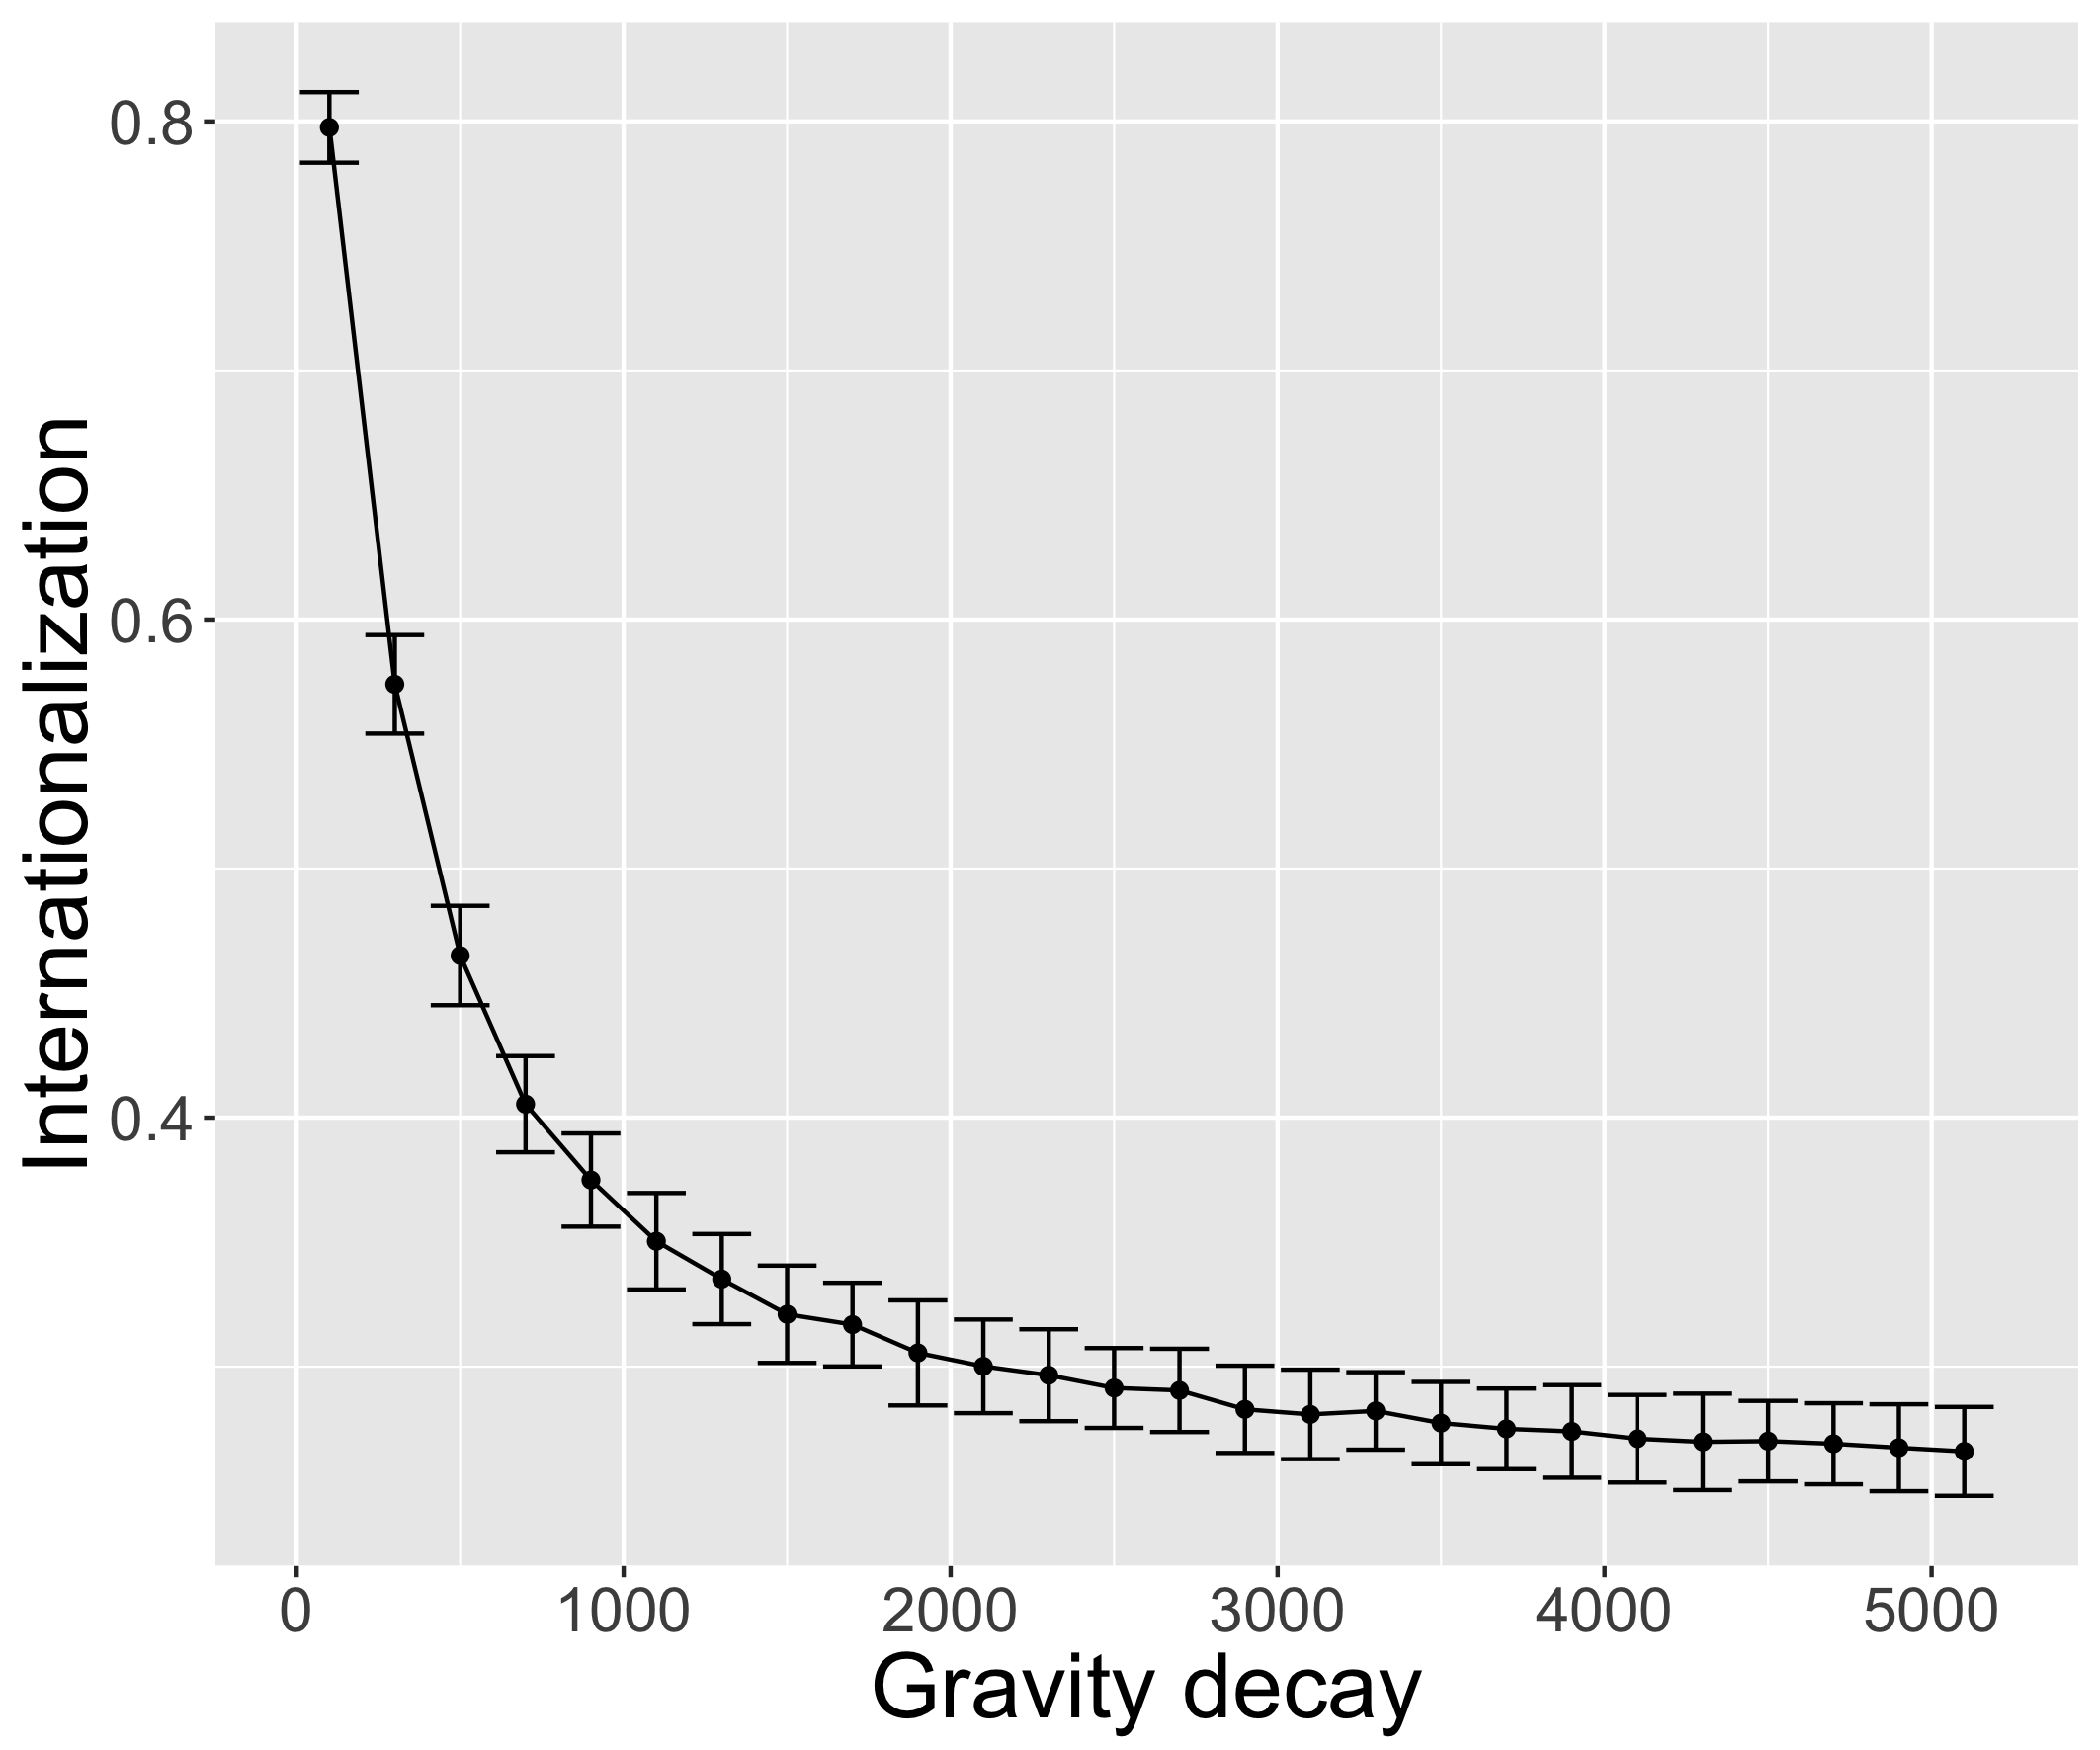
\includegraphics[width=0.48\textwidth,height=0.25\textheight]{figures/internationalization-gravityDecay_errorbars.png}
    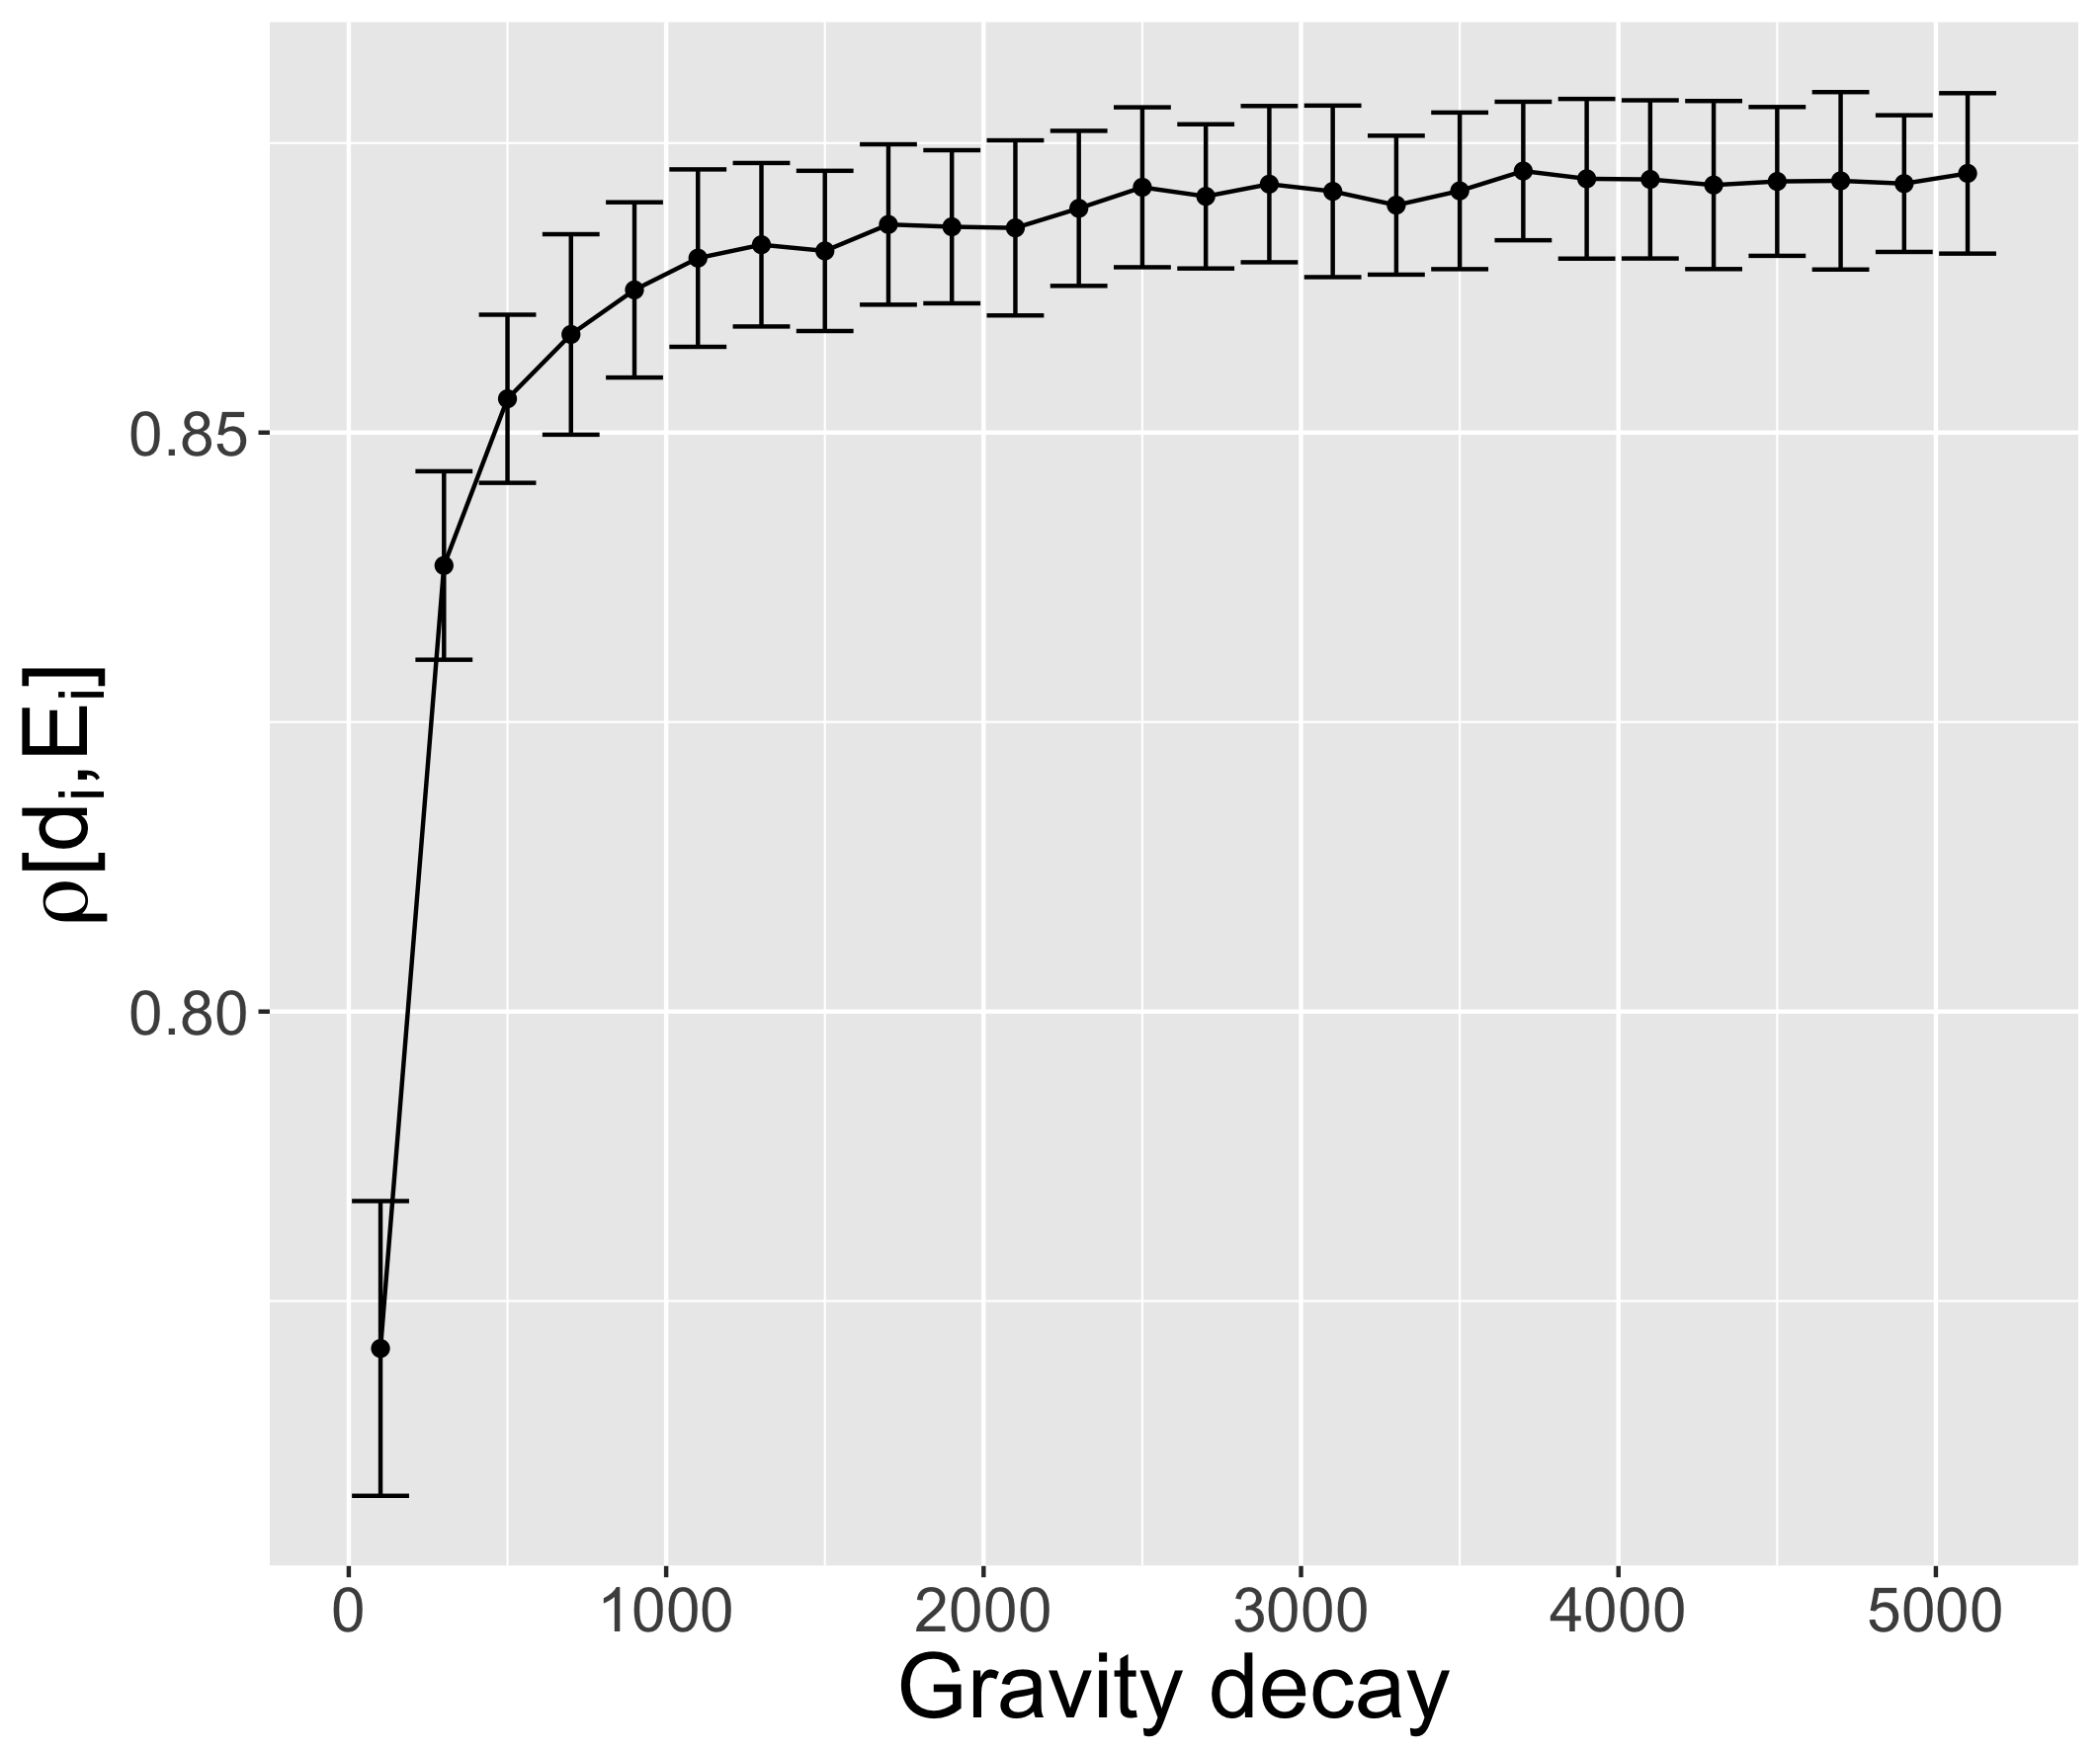
\includegraphics[width=0.48\textwidth,height=0.25\textheight]{figures/rhoDegreeSize-gravityDecay_errorbars.png}\\
    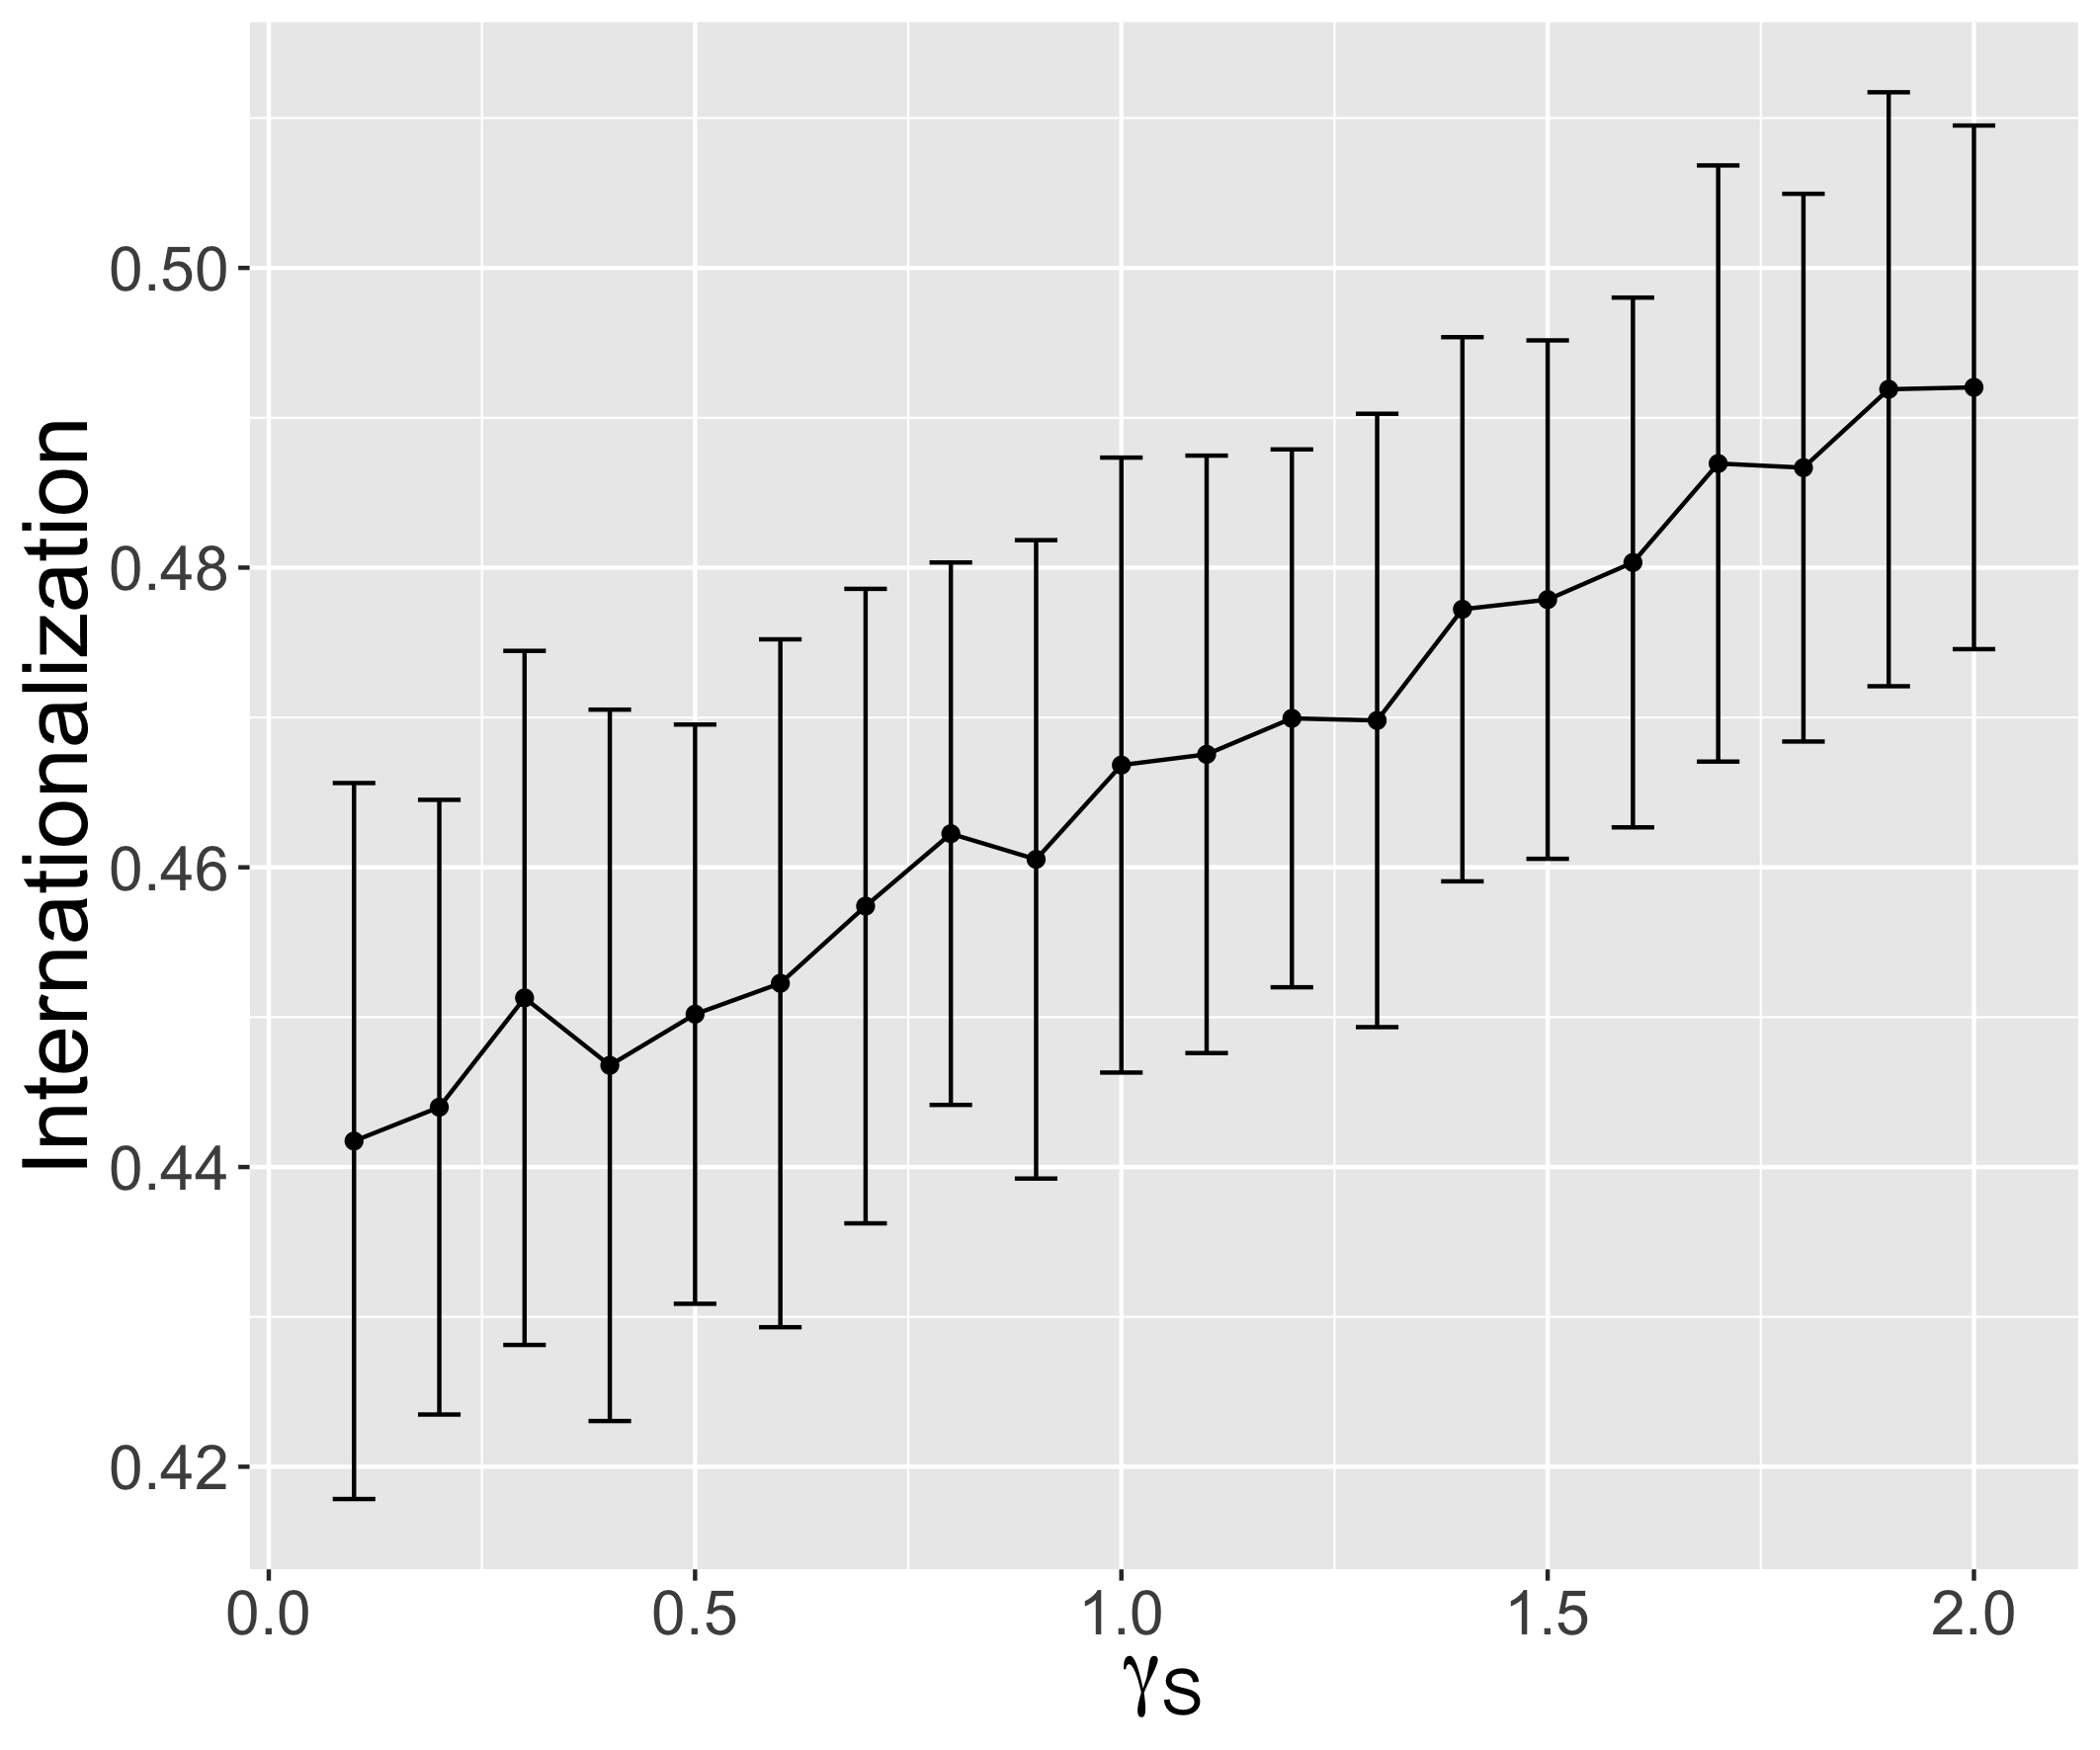
\includegraphics[width=0.48\textwidth,height=0.25\textheight]{figures/internationalization-gammaSectors_errorbars.png}
    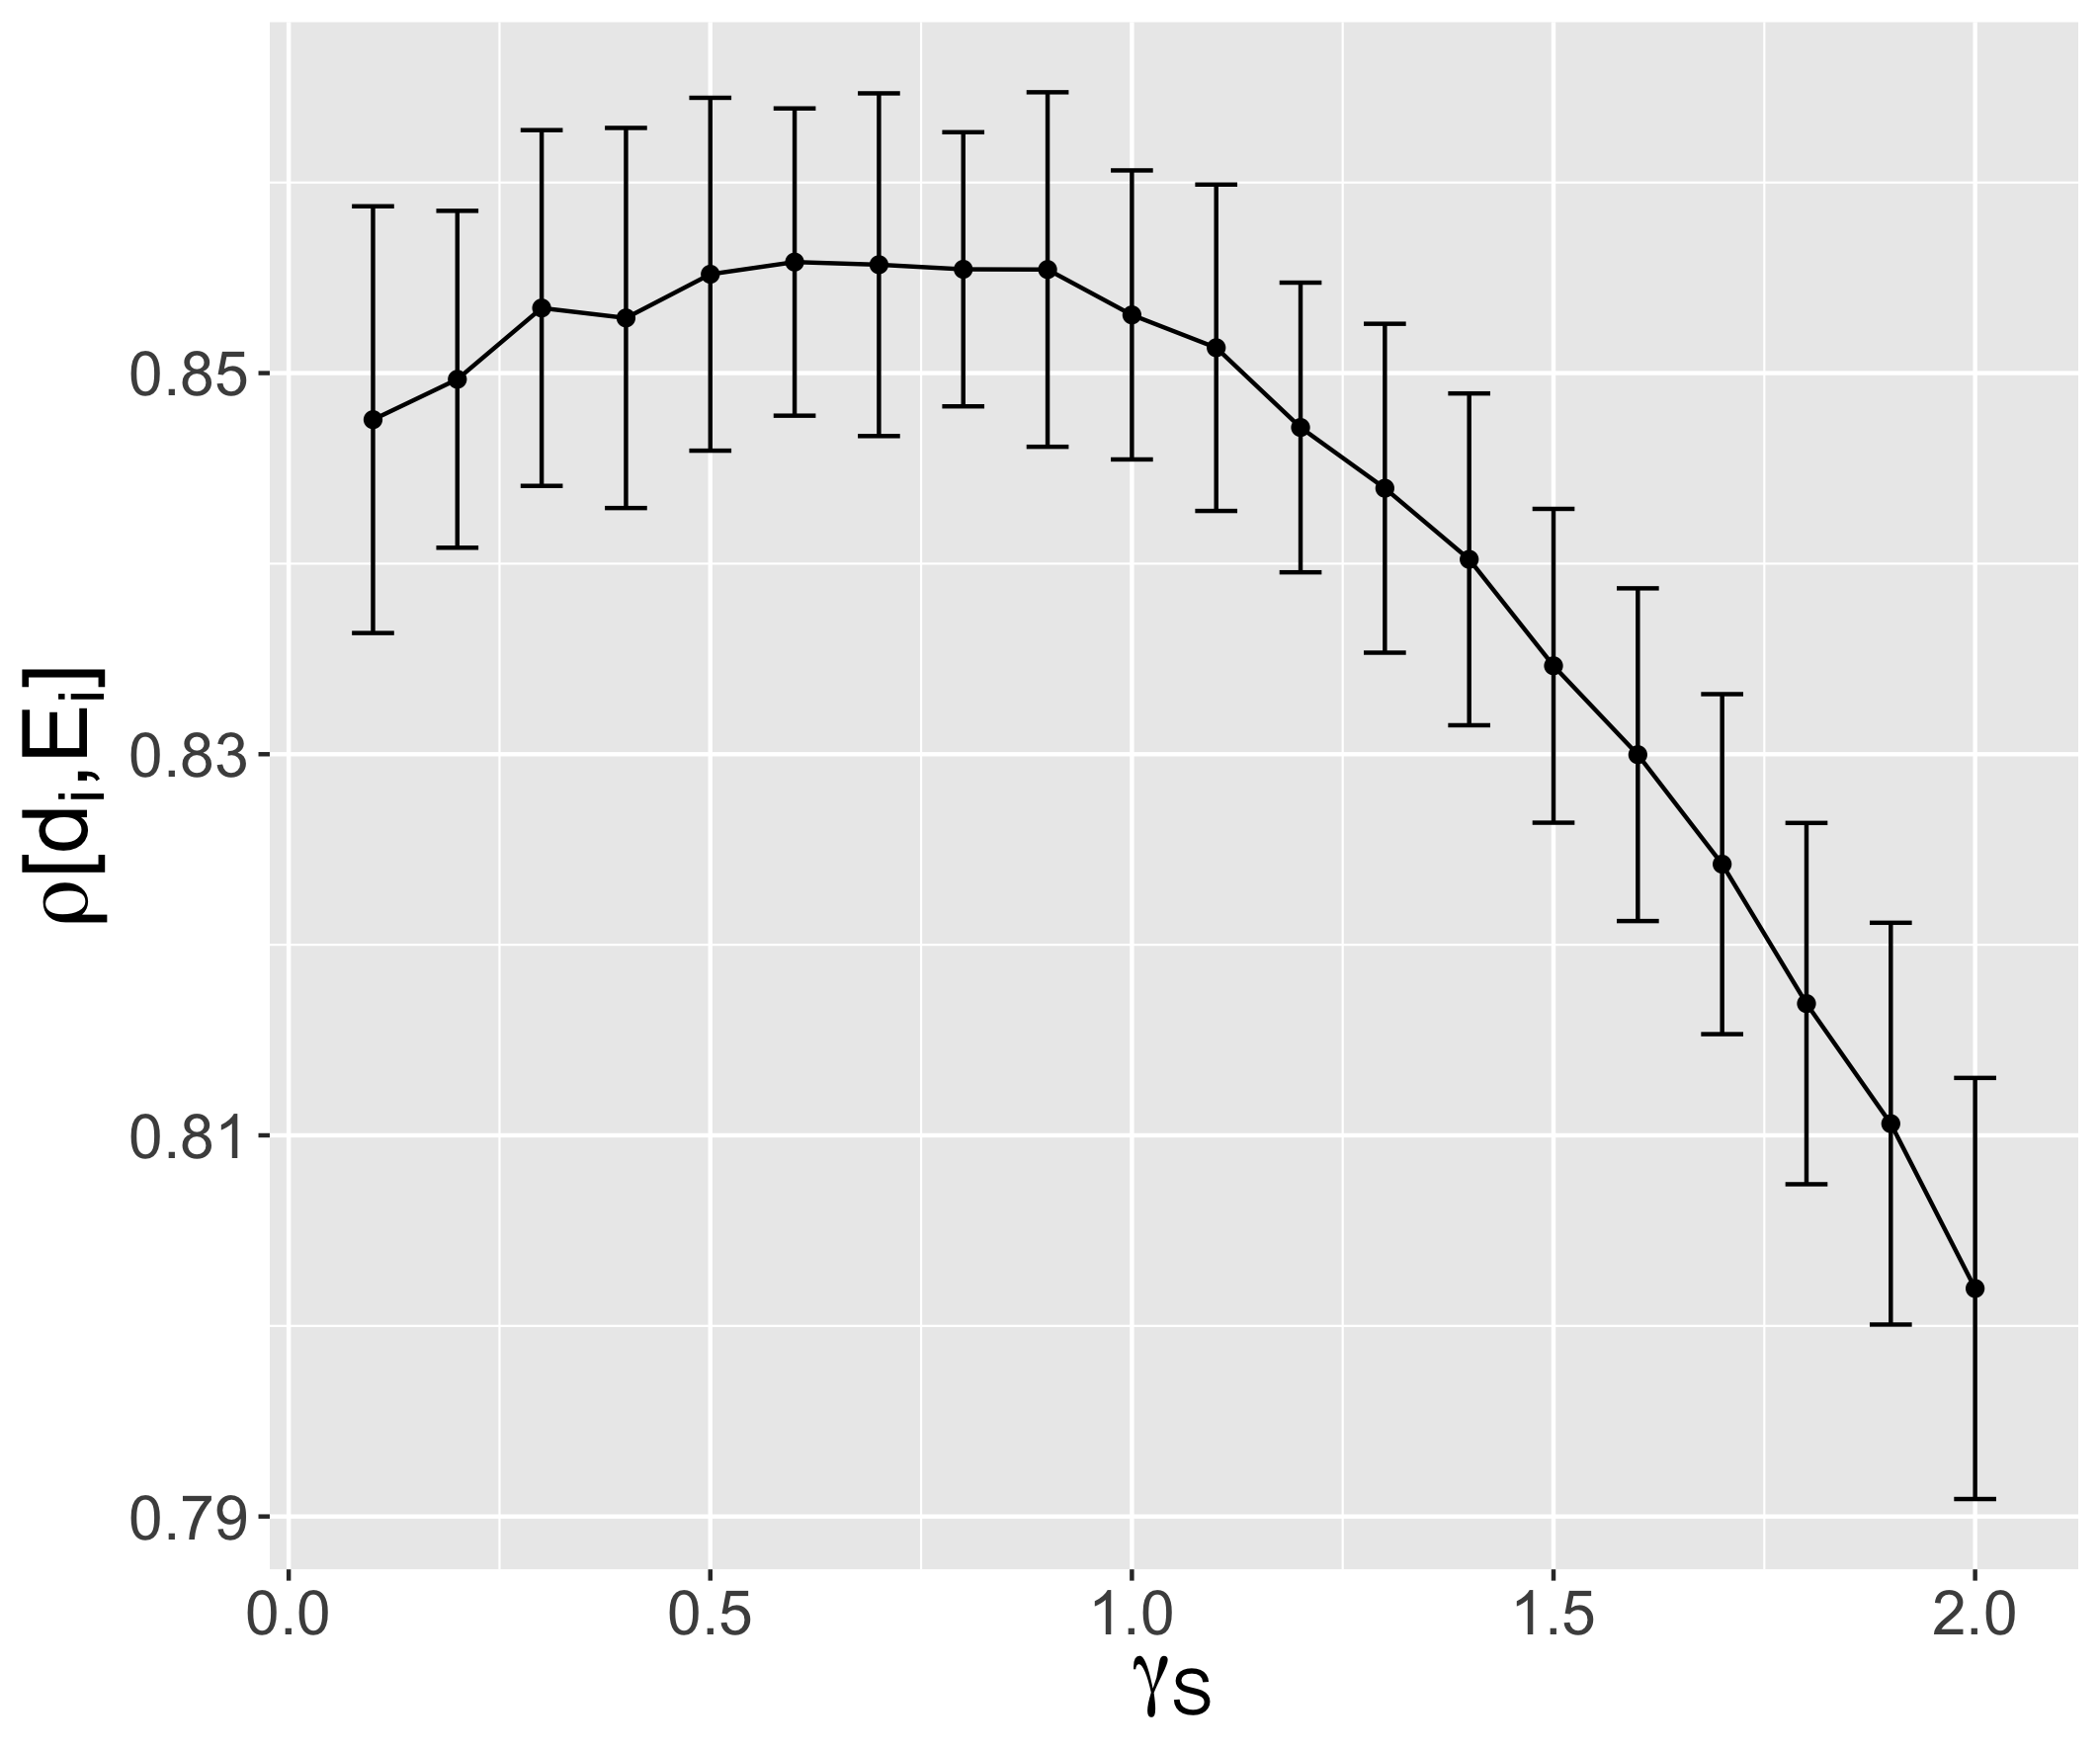
\includegraphics[width=0.48\textwidth,height=0.25\textheight]{figures/rhoDegreeSize-gammaSectors_errorbars.png}
    \caption{(Top Left) Internationalisation index decreases exponentially with gravity decay; (Top Right) Correlation between city weighted degree and size. Both plots show a transition from a local to a global regime. (Bottom Left) Internationalisation varies linearly with sector proximity $\gamma_S$; (Bottom Right) Correlation between degree and size exhibits a maximum, witnessing an intermediate regime where size is the most important. \label{fig:onefactor}}
\end{figure}
%%%%%%%%%%%%%



\paragraph{Grid exploration}

The model behaviour is then studied with a grid sampling for parameters and 20 repetitions (the computations run on the European Grid Infrastructure, and are equivalent to 2.5 years of CPU time). Distance decay and sector  parameters are varied with 10 steps, other parameters with three. The influence of gravity decay parameters is confirmed when plotting the internationalization index against the distance, which exhibits an exponential decay as shown in Fig.~\ref{fig:internat}. It interacts with the role of sectors and the size of the origin, with a more significant effect of sector proximity when size has the largest influence (third panel).


%%%%%%%%%%%%%%
\begin{figure}
    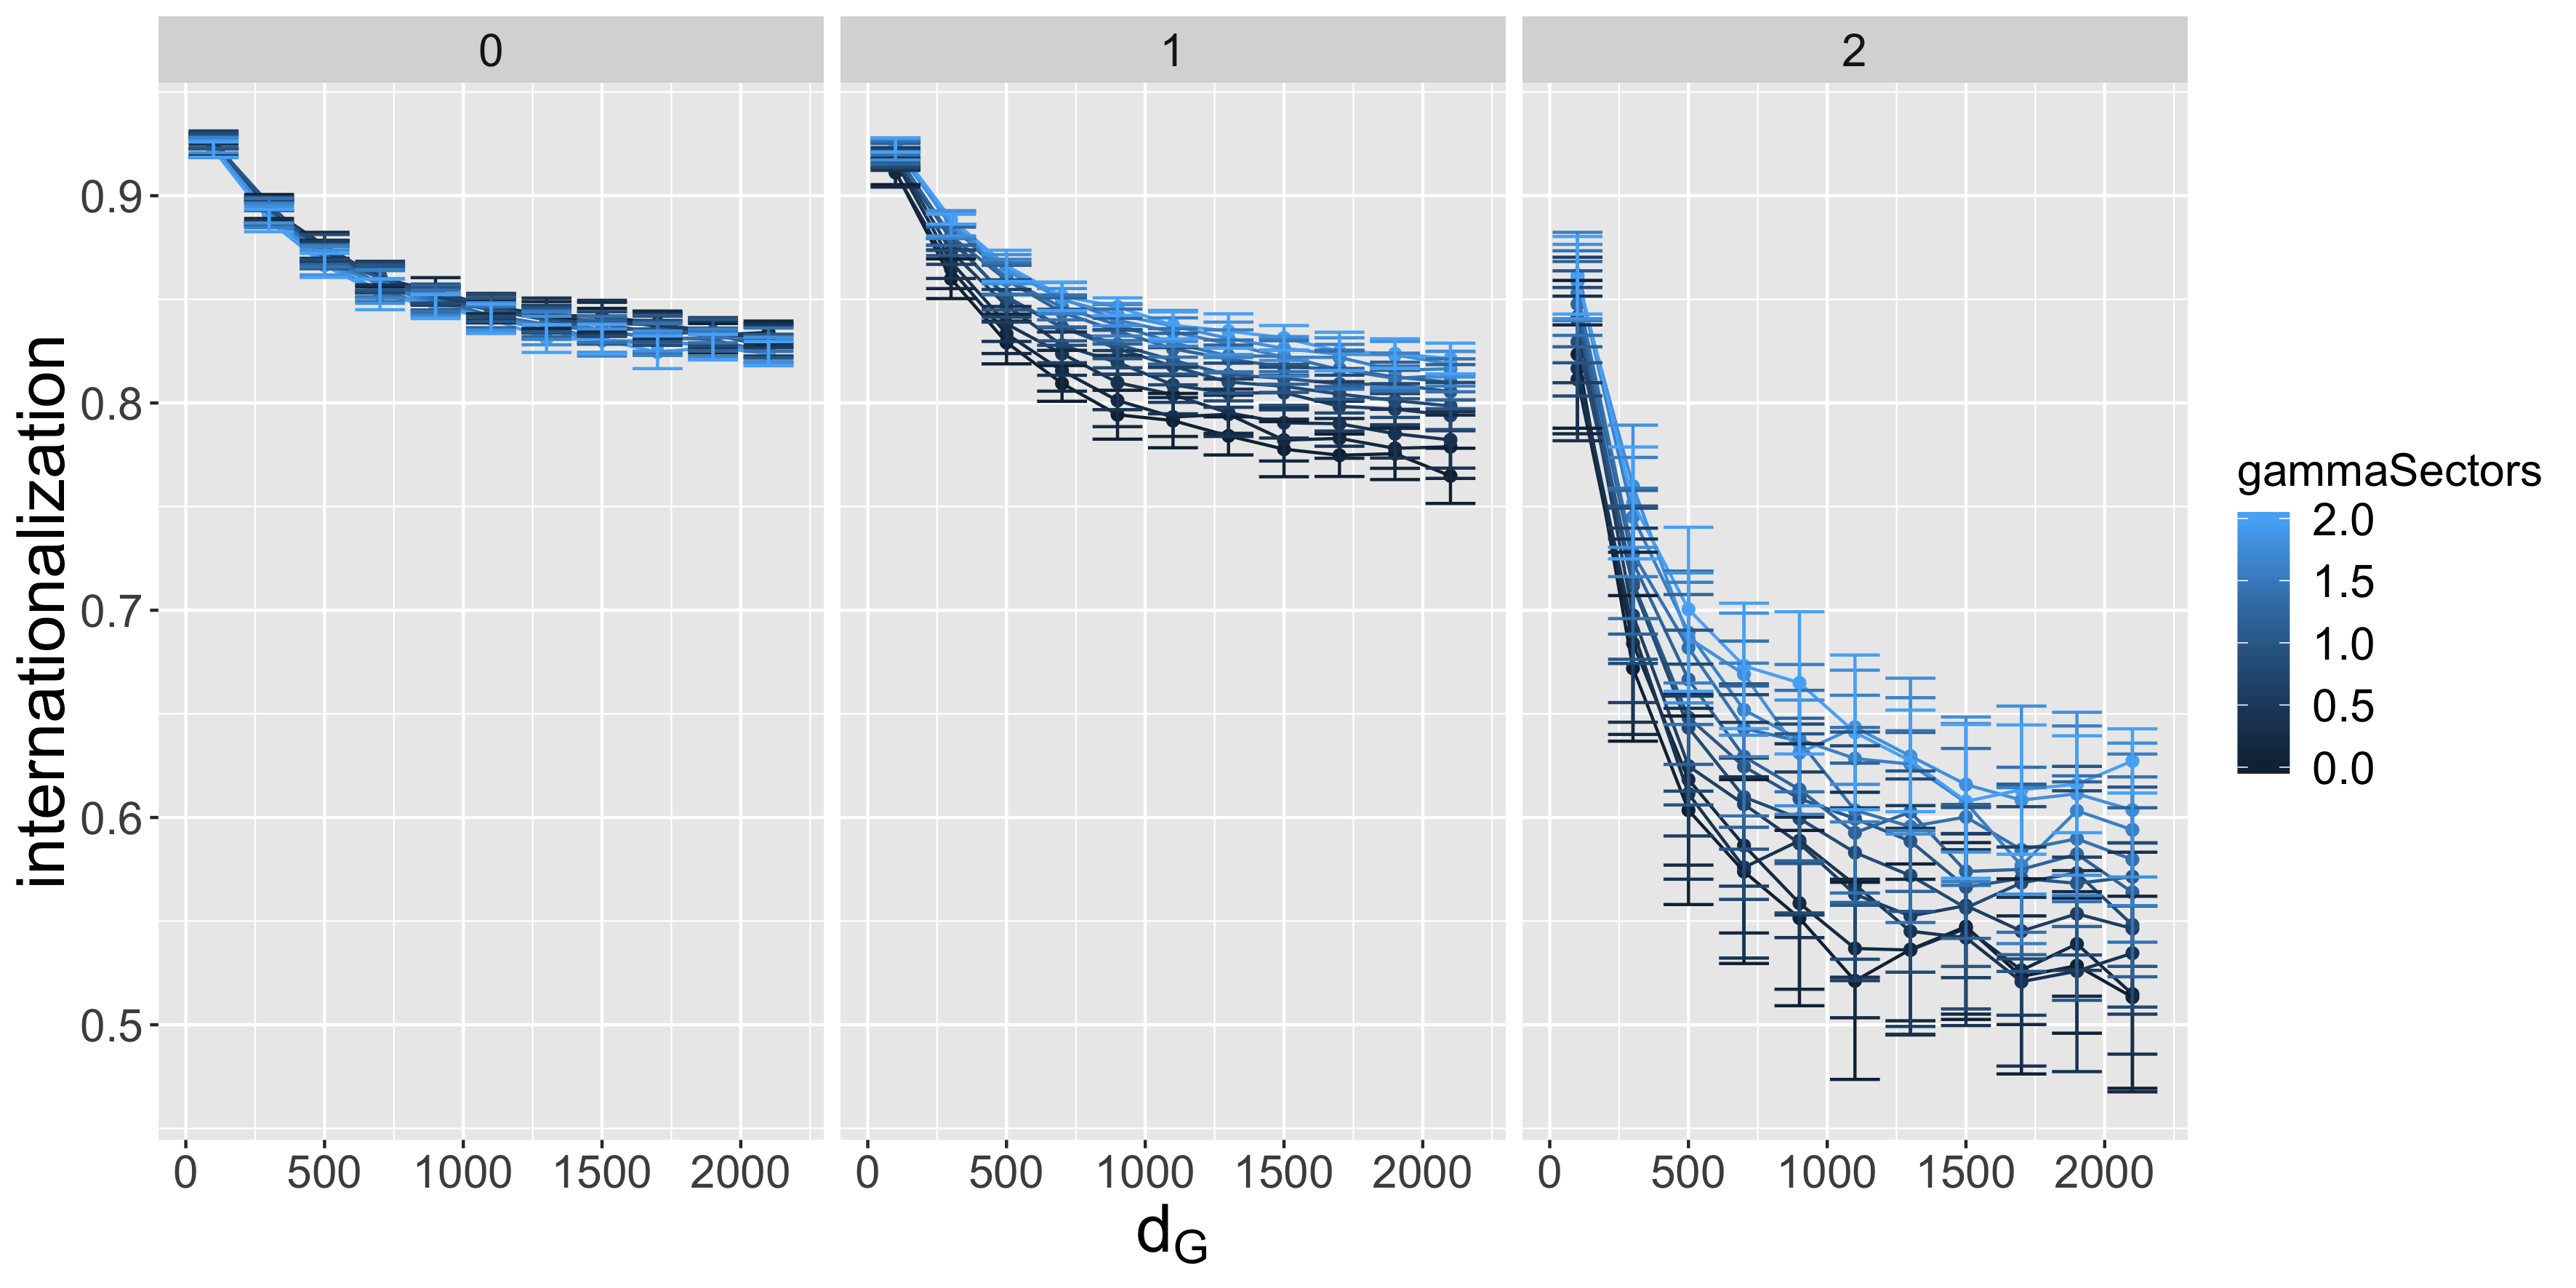
\includegraphics[width=\textwidth]{figures/internationalization_countryGravityDecay200_gammaDestination0_facetwrapgammaOrigin_colorgammaSectors.png}
    \caption{The transition as a function of interaction range depends on the influence of origin size $\gamma_F$; sector proximity $\gamma_S$ plays a role only for a large influence of the origin.\label{fig:internat}}
\end{figure}
%%%%%%%%%%%%%%


Other indicators exhibit non-trivial patterns. For example, when considering average community size of the final network as shown in Fig.~\ref{fig:comsize}, we obtain a maximal integration in term of communities at an intermediate value of the gravity decay, what can be interpreted as the emergence of a regional regime. The size of communities is largely influenced by the value of the elasticities for the similarity function and the ratio of the economic output of the area. In particular, we observe a qualitative inversion of the role of $\gamma_S$ when introducing an effect of the origin (switching $\gamma_F$ from 0 to 1, first panel to second panel). The maximal community size disappears when $\gamma_F = 2$, implying a regime with small local communities where large cities mostly connect with there hinterland. These experiments reveal a complex interplay between processes and how the model produces diverse stylised facts.

%%%%%%%%%%%%%%
\begin{figure}
    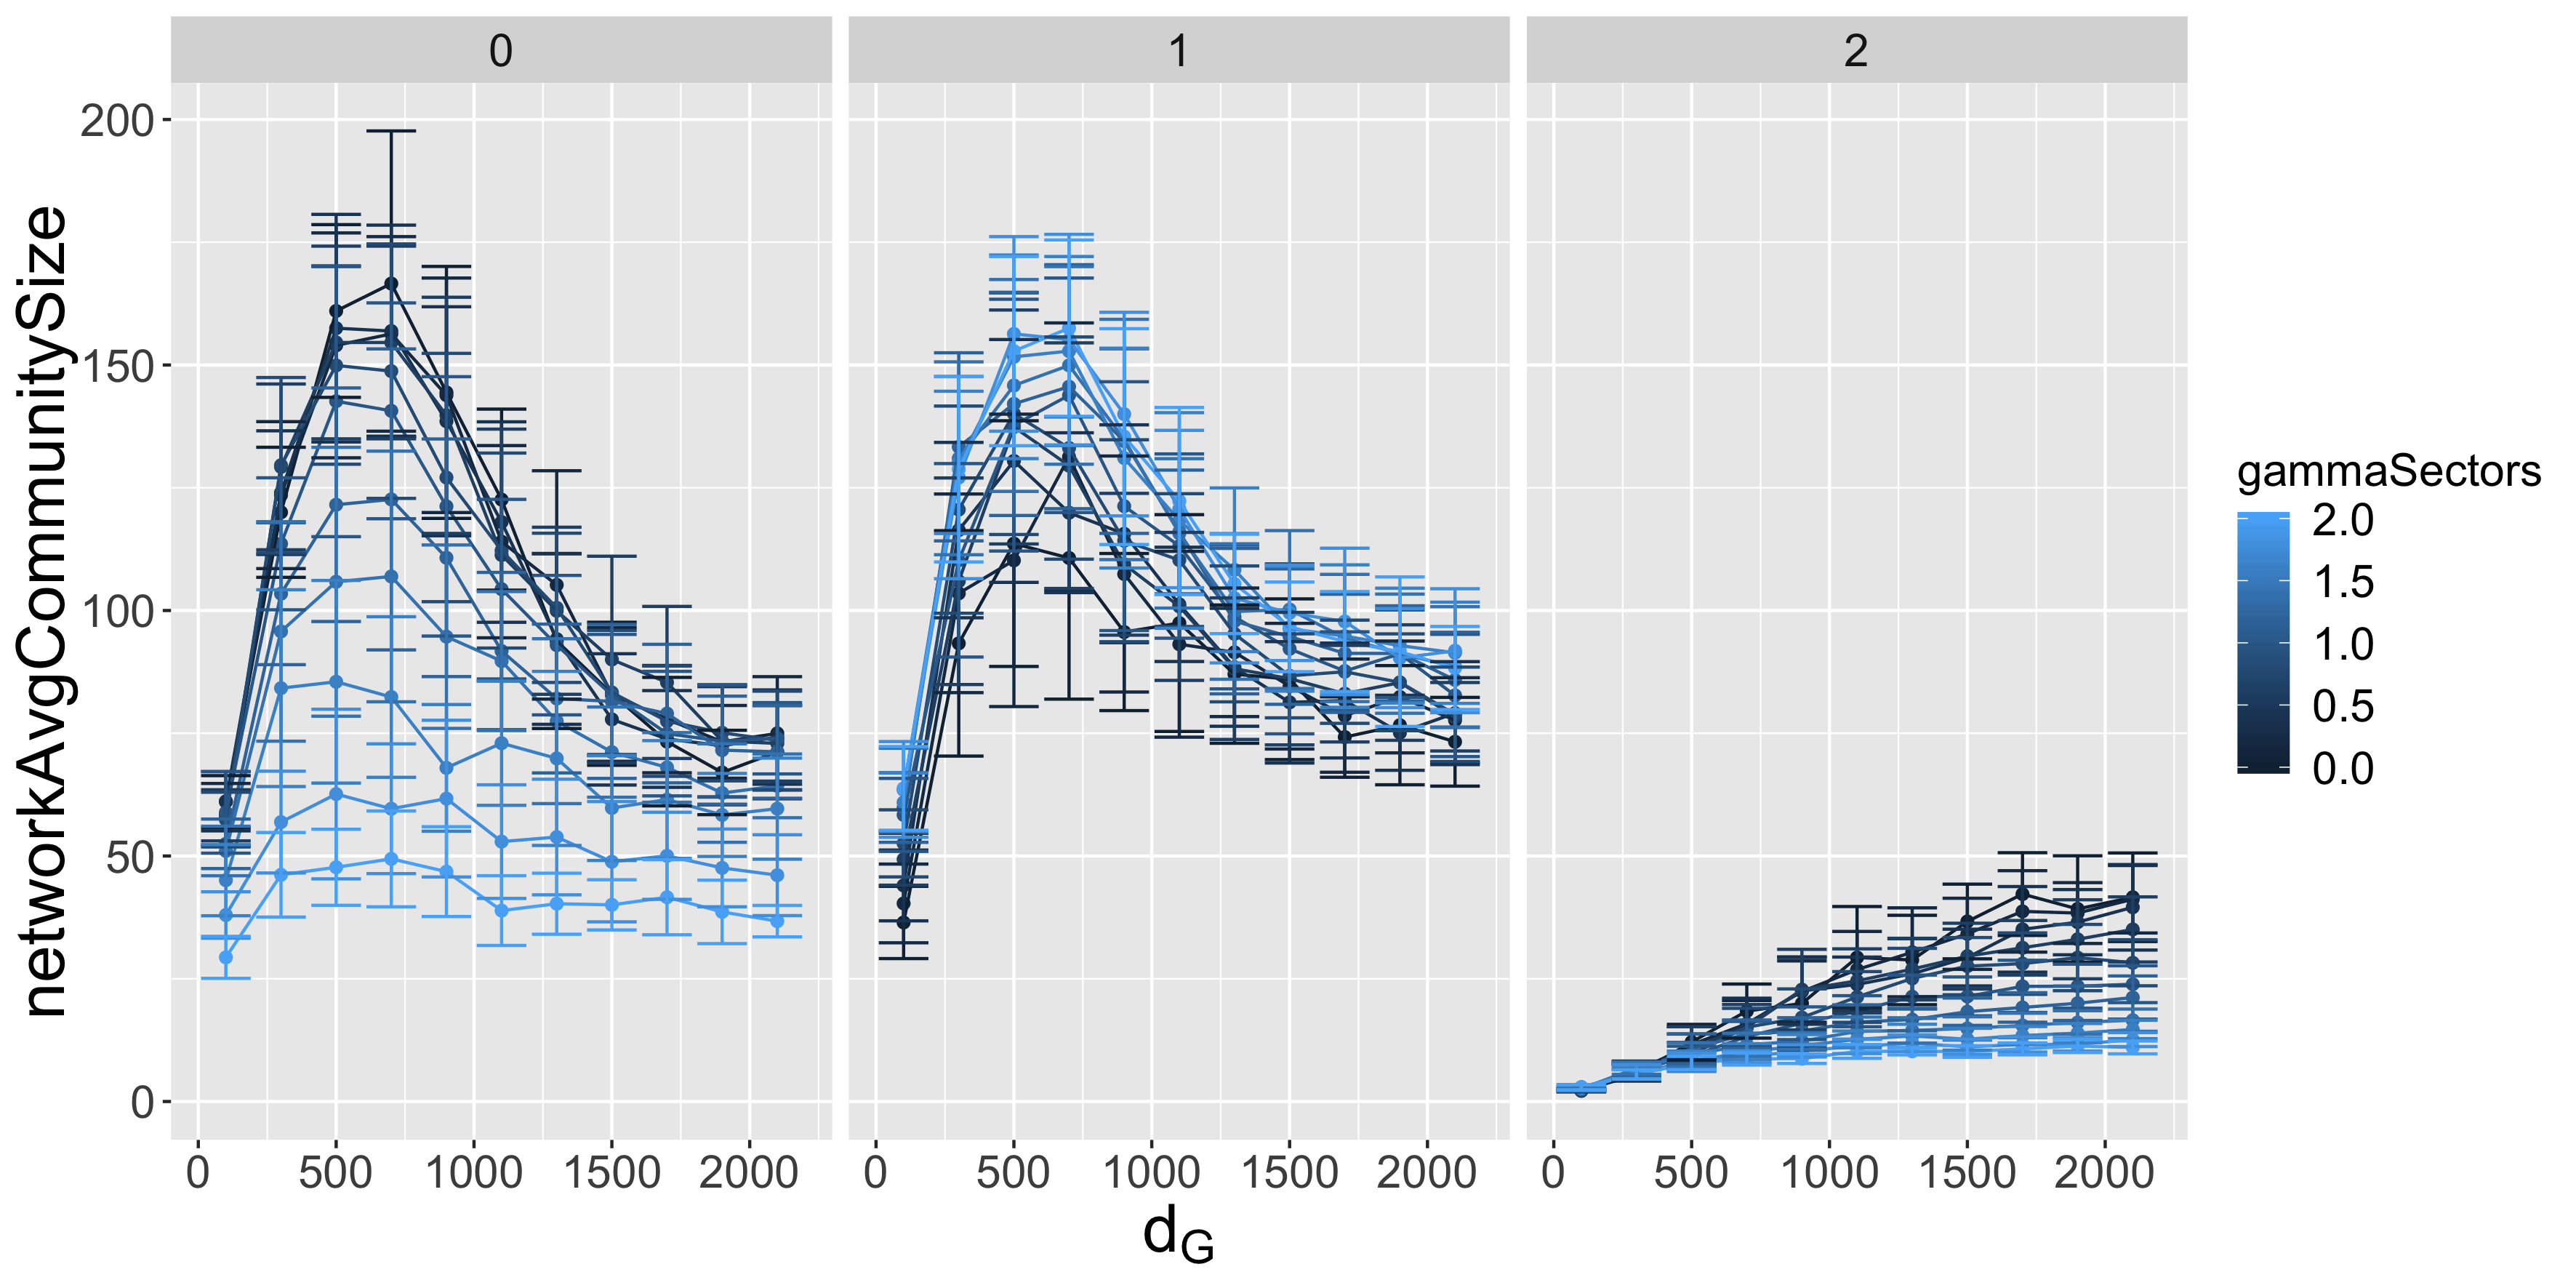
\includegraphics[width=\textwidth]{figures/networkAvgCommunitySize_countryGravityDecay2100_gammaDestination0_facetwrapgammaOrigin_colorgammaSectors.png}
	\caption{Maximal integration in term of community size is achieved at an intermediate value of $d_G$: emergence of a regional regime; Maximal size depends on the role of sectors $\gamma_S$, in a decreasing way when origin size is deactivated, and increasing way when $\gamma_F=1$; This regime disappear when origin size influence is too large.\label{fig:comsize}}
\end{figure}
%%%%%%%%%%%%%%




\subsection{Model calibration on the European urban network}


We then apply the model to a real system of cities by calibrating it on the European ownership network. Model setup is done following the real setup described above. The number of time steps $t_f$ is left as an additional parameter, which in a sense determines the granularity of the cumulative network generation process. The objective functions for calibration are the average mean squared error on logarithms of weights given by $\varepsilon_L = \frac{1}{N^2} \sum_{i,j} \left(\log w_{ij} - \log \hat{w}_{ij} \right)^2$ if $\hat{w}_{ij}$ are the simulated weights, and the logarithm of the mean squared error $\varepsilon_M = \log\left(\frac{1}{N^2} \sum_{i,j} \left(w_{ij} - \hat{w}_{ij}\right)^2 \right)$. \cite{raimbault2018indirect} showed that these two are complementary to calibrate urban systems models. Calibration is done using a genetic NSGA2 algorithm \cite{deb2002fast}, which is particularly suited for such a bi-objective calibration of a stochastic simulation model. We use a population of 200 and run the algorithm for 20,000 generations, on 1000 islands in parallel.


%%%%%%%%%%%%%%
\begin{figure}
	\begin{center}
    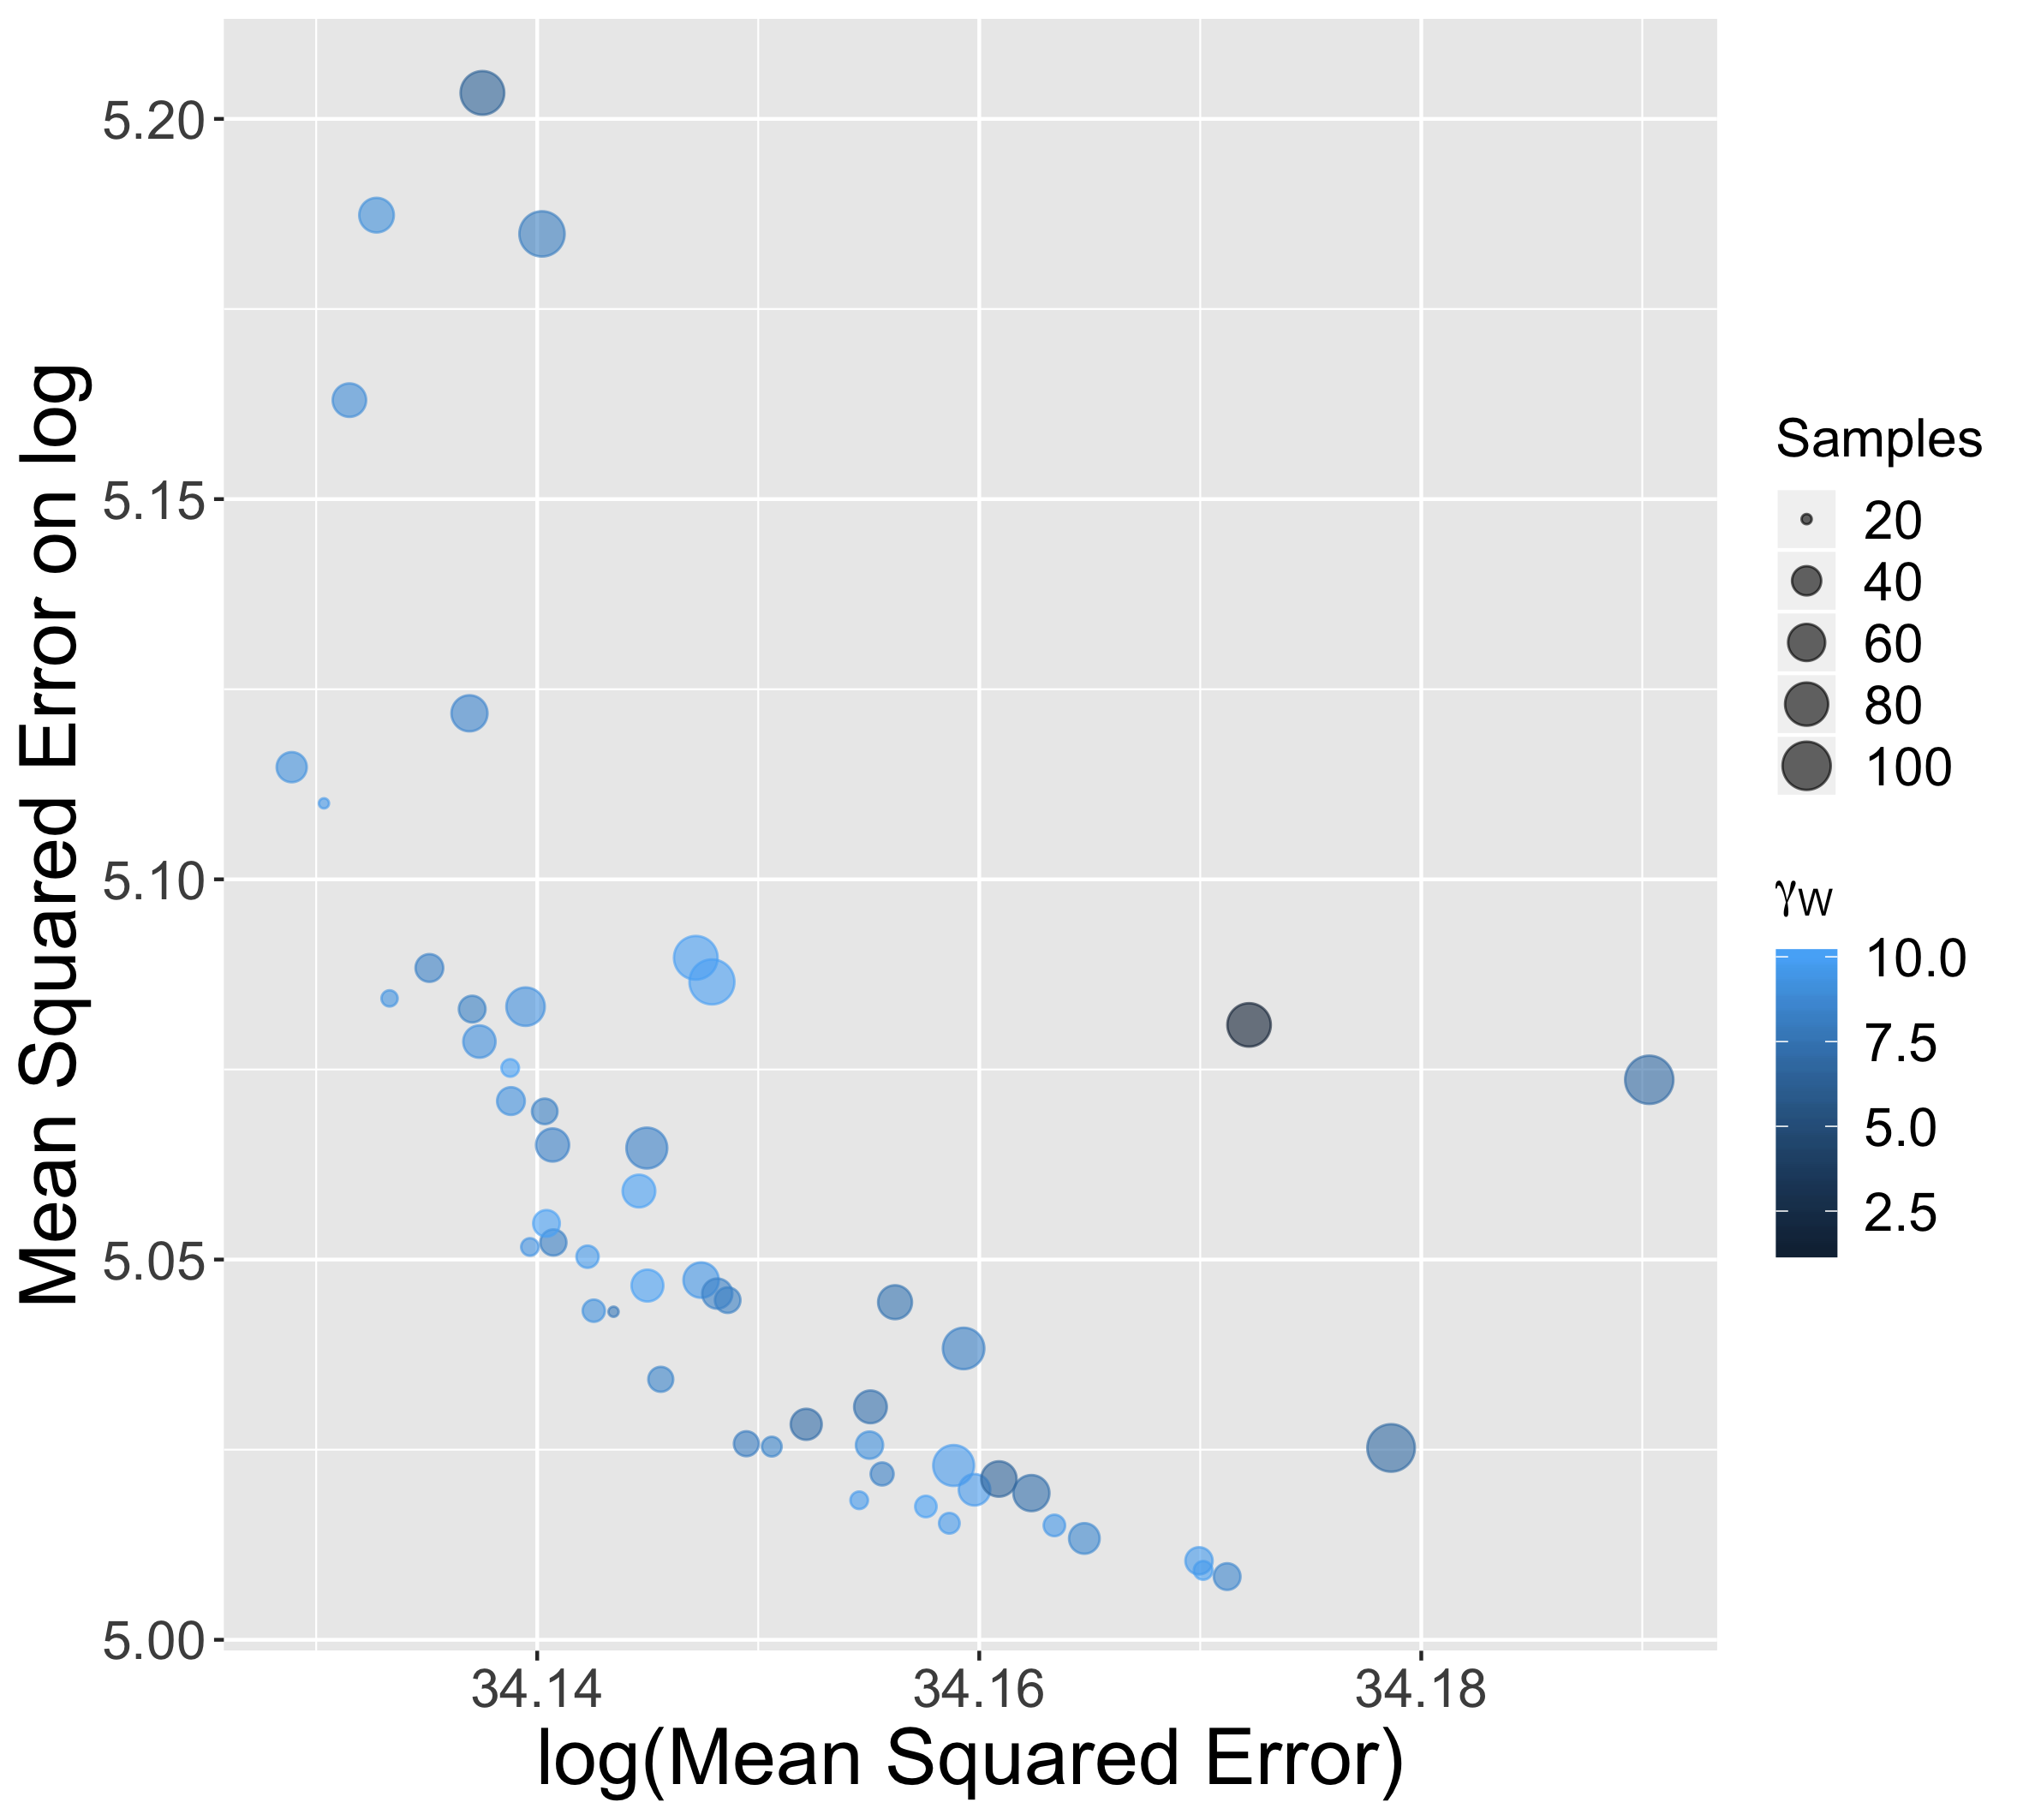
\includegraphics[width=0.5\textwidth]{figures/pareto_colorgammaLinks.png}
    \end{center}
	\caption{Pareto front obtained for the bi-objective model calibration.\label{fig:calibration}}
\end{figure}
%%%%%%%%%%%%%%


We show in Fig.~\ref{fig:calibration} the calibration result, as a Pareto front of compromise points between the two objectives. These correspond to parameter values giving network trajectories closest to reality. The values for $\varepsilon_L$ are always lower than for statistical models, our model outperforming these in this predictive sense.
% add discussion param values
This furthermore shows in particular a role of the path-dependency parameter, which calibrated value is quite high (8 in average on the Pareto front), confirming the relevance of this complex generative model including path-dependency. These results altogether demonstrate the feasibility of model calibration on real data.


%%%%%%%%%%%%%%%
\section{Discussion}

This paper aimed at presenting a generative model for urban networks defined by interactions between firms based on synthetic data, simulated via the OpenMole platform and calibrated on real data on ownership linkages of firms for Europe. The simulation on a synthetic system of cities unveil phase transitions when changing interaction distance, and non-trivial patterns in the model behavior. This kind of model can have practical application in the future in terms of testing the effect of exogenous shocks in the socio-economic structure as the upcoming effect of Brexit on the European market.

Even in such a simple model (close to directly tractable stationary state) the behaviour is highly non-linear in many dimensions. Our study shows how crucial model exploration is to overcome hidden parameters (deactivated mechanisms or default parameter values). This paper emphasis on the fact that exploration of intrinsic dynamics on synthetic data is of great importance should be driven before an application on real data so as to put aside the geographical effects from model dynamics.

Several possible extensions of the current work can be undertaken in the future as a co-evolution model with an evolution of city sizes or a model with firm agents leading to a multi-scale agent-based model. A more precise study of the role of path dependency can also be undertaken in order to understand the creation of the future links. Other formulations of the model might be taken into consideration as other formulation of the combination of factors or multi-objective optimisation depending on sectors using Pareto fronts.  


% Several scenarios are considered taking into consideration the current and future economic challenges, such as those given by Brexit. The model may be applied in future work to assess policy issues and recommendations.

% - other formulation of the combination of factors
%multi-objective optimisation depending on sectors, using Pareto fronts ? - needs empirical evidence; (iv) copula-based combination as done by \cite{2019arXiv190505106C} - copula parameters are free or estimated from real data
% The function used can be understood as a separable spatial interaction model. As a possible extension, Copula capture a dependency structure but must be parametrised by estimation on real data.

% - evolution of city sizes (co-evolution model)
% - role of path dependency
% - towards a model with firm agents? (multi-scale ABM)


%\bibliographystyle{apalike}
\bibliographystyle{unsrt}
\bibliography{biblio}

\end{document}
